
%% IAENG_pub.tex 2010/08/30
%% It is based on the bare_jrnl.tex V1.3 2007/01/11 by Michael Shell
%% see http://www.michaelshell.org/
%% for current contact information.
%%
%% This is a skeleton file demonstrating the use of IAENGtran.cls
%% (requires IAENGtran.cls version 1.7 or later) with an IAENG journal/conference paper.
%%
%% Support sites:
%% http://www.michaelshell.org/tex
%% http://www.ctan.org/tex-archive/macros/latex/contrib/IEEEtran/

% *** Authors should verify (and, if needed, correct) their LaTeX system  ***
% *** with the testflow diagnostic prior to trusting their LaTeX platform ***
% *** with production work. IAENG's font choices can trigger bugs that do  ***
% *** not appear when using other class files.                            ***
% The testflow support page is at:
% http://www.michaelshell.org/tex/testflow/


%%*************************************************************************
%% Legal Notice:
%% This code is offered as-is without any warranty either expressed or
%% implied; without even the implied warranty of MERCHANTABILITY or
%% FITNESS FOR A PARTICULAR PURPOSE!
%% User assumes all risk.
%% In no event shall IAENG or any contributor to this code be liable for
%% any damages or losses, including, but not limited to, incidental,
%% consequential, or any other damages, resulting from the use or misuse
%% of any information contained here.
%%
%% All comments are the opinions of their respective authors and are not
%% necessarily endorsed by the IAENG.
%%
%% This work is distributed under the LaTeX Project Public License (LPPL)
%% ( http://www.latex-project.org/ ) version 1.3, and may be freely used,
%% distributed and modified. A copy of the LPPL, version 1.3, is included
%% in the base LaTeX documentation of all distributions of LaTeX released
%% 2003/12/01 or later.
%% Retain all contribution notices and credits.
%% ** Modified files should be clearly indicated as such, including  **
%% ** renaming them and changing author support contact information. **
%%
%%*************************************************************************

% Note that the a4paper option is mainly intended so that authors in
% countries using A4 can easily print to A4 and see how their papers will
% look in print - the typesetting of the document will not typically be
% affected with changes in paper size (but the bottom and side margins will).
% Use the testflow package mentioned above to verify correct handling of
% both paper sizes by the user's LaTeX system.
%
% Also note that the "draftcls" or "draftclsnofoot", not "draft", option
% should be used if it is desired that the figures are to be displayed in
% draft mode.
%
\documentclass[journal]{IAENGtran}
%
% If IAENGtran.cls has not been installed into the LaTeX system files,
% manually specify the path to it like:
% \documentclass[journal]{../sty/IAENGtran}





% Some very useful LaTeX packages include:
% (uncomment the ones you want to load)


% *** MISC UTILITY PACKAGES ***
%
%\usepackage{ifpdf}
% Heiko Oberdiek's ifpdf.sty is very useful if you need conditional
% compilation based on whether the output is pdf or dvi.
% usage:
% \ifpdf
%   % pdf code
% \else
%   % dvi code
% \fi
% The latest version of ifpdf.sty can be obtained from:
% http://www.ctan.org/tex-archive/macros/latex/contrib/oberdiek/
% Also, note that IAENGtran.cls V1.7 and later provides a builtin
% \ifCLASSINFOpdf conditional that works the same way.
% When switching from latex to pdflatex and vice-versa, the compiler may
% have to be run twice to clear warning/error messages.






% *** CITATION PACKAGES ***
%
%\usepackage{cite}
% cite.sty was written by Donald Arseneau
% V1.6 and later of IAENGtran pre-defines the format of the cite.sty package
% \cite{} output to follow that of IAENG. Loading the cite package will
% result in citation numbers being automatically sorted and properly
% "compressed/ranged". e.g., [1], [9], [2], [7], [5], [6] without using
% cite.sty will become [1], [2], [5]--[7], [9] using cite.sty. cite.sty's
% \cite will automatically add leading space, if needed. Use cite.sty's
% noadjust option (cite.sty V3.8 and later) if you want to turn this off.
% cite.sty is already installed on most LaTeX systems. Be sure and use
% version 4.0 (2003-05-27) and later if using hyperref.sty. cite.sty does
% not currently provide for hyperlinked citations.
% The latest version can be obtained at:
% http://www.ctan.org/tex-archive/macros/latex/contrib/cite/
% The documentation is contained in the cite.sty file itself.






% *** GRAPHICS RELATED PACKAGES ***
%
\ifCLASSINFOpdf
   \usepackage[pdftex]{graphicx}
  % declare the path(s) where your graphic files are
   \graphicspath{{../figures/}}
  % and their extensions so you won't have to specify these with
  % every instance of \includegraphics
   \DeclareGraphicsExtensions{.pdf,.jpeg,.png}
\else
  % or other class option (dvipsone, dvipdf, if not using dvips). graphicx
  % will default to the driver specified in the system graphics.cfg if no
  % driver is specified.
   \usepackage[dvips]{graphicx}
  % declare the path(s) where your graphic files are
   \graphicspath{{../figures/}}
  % and their extensions so you won't have to specify these with
  % every instance of \includegraphics
   \DeclareGraphicsExtensions{.eps}
\fi
% graphicx was written by David Carlisle and Sebastian Rahtz. It is
% required if you want graphics, photos, etc. graphicx.sty is already
% installed on most LaTeX systems. The latest version and documentation can
% be obtained at:
% http://www.ctan.org/tex-archive/macros/latex/required/graphics/
% Another good source of documentation is "Using Imported Graphics in
% LaTeX2e" by Keith Reckdahl which can be found as epslatex.ps or
% epslatex.pdf at: http://www.ctan.org/tex-archive/info/
%
% latex, and pdflatex in dvi mode, support graphics in encapsulated
% postscript (.eps) format. pdflatex in pdf mode supports graphics
% in .pdf, .jpeg, .png and .mps (metapost) formats. Users should ensure
% that all non-photo figures use a vector format (.eps, .pdf, .mps) and
% not a bitmapped formats (.jpeg, .png). IAENG frowns on bitmapped formats
% which can result in "jaggedy"/blurry rendering of lines and letters as
% well as large increases in file sizes.
%
% You can find documentation about the pdfTeX application at:
% http://www.tug.org/applications/pdftex



% *** MATH PACKAGES ***
%
\usepackage[cmex10]{amsmath}
% A popular package from the American Mathematical Society that provides
% many useful and powerful commands for dealing with mathematics. If using
% it, be sure to load this package with the cmex10 option to ensure that
% only type 1 fonts will utilized at all point sizes. Without this option,
% it is possible that some math symbols, particularly those within
% footnotes, will be rendered in bitmap form which will result in a
% document that can not be IAENG compliant!
%
% Also, note that the amsmath package sets \interdisplaylinepenalty to 10000
% thus preventing page breaks from occurring within multiline equations. Use:
%\interdisplaylinepenalty=2500
% after loading amsmath to restore such page breaks as IAENGtran.cls normally
% does. amsmath.sty is already installed on most LaTeX systems. The latest
% version and documentation can be obtained at:
% http://www.ctan.org/tex-archive/macros/latex/required/amslatex/math/





% *** SPECIALIZED LIST PACKAGES ***
%
%\usepackage{algorithmic}
% algorithmic.sty was written by Peter Williams and Rogerio Brito.
% This package provides an algorithmic environment for describing algorithms.
% You can use the algorithmic environment in-text or within a figure
% environment to provide for a floating algorithm. Do NOT use the algorithm
% floating environment provided by algorithm.sty (by the same authors) or
% algorithm2e.sty (by Christophe Fiorio) as IAENG does not use dedicated
% algorithm float types and packages that provide these will not provide
% correct IAENG style captions. The latest version and documentation of
% algorithmic.sty can be obtained at:
% http://www.ctan.org/tex-archive/macros/latex/contrib/algorithms/
% There is also a support site at:
% http://algorithms.berlios.de/index.html
% Also of interest may be the (relatively newer and more customizable)
% algorithmicx.sty package by Szasz Janos:
% http://www.ctan.org/tex-archive/macros/latex/contrib/algorithmicx/




% *** ALIGNMENT PACKAGES ***
%
%\usepackage{array}
% Frank Mittelbach's and David Carlisle's array.sty patches and improves
% the standard LaTeX2e array and tabular environments to provide better
% appearance and additional user controls. As the default LaTeX2e table
% generation code is lacking to the point of almost being broken with
% respect to the quality of the end results, all users are strongly
% advised to use an enhanced (at the very least that provided by array.sty)
% set of table tools. array.sty is already installed on most systems. The
% latest version and documentation can be obtained at:
% http://www.ctan.org/tex-archive/macros/latex/required/tools/


%\usepackage{mdwmath}
%\usepackage{mdwtab}
% Also highly recommended is Mark Wooding's extremely powerful MDW tools,
% especially mdwmath.sty and mdwtab.sty which are used to format equations
% and tables, respectively. The MDWtools set is already installed on most
% LaTeX systems. The lastest version and documentation is available at:
% http://www.ctan.org/tex-archive/macros/latex/contrib/mdwtools/


% IAENGtran contains the IAENGeqnarray family of commands that can be used to
% generate multiline equations as well as matrices, tables, etc., of high
% quality.


%\usepackage{eqparbox}
% Also of notable interest is Scott Pakin's eqparbox package for creating
% (automatically sized) equal width boxes - aka "natural width parboxes".
% Available at:
% http://www.ctan.org/tex-archive/macros/latex/contrib/eqparbox/

\usepackage{tabularx}
\usepackage{multirow}
\usepackage{booktabs}

\newcolumntype{Y}{>{\centering\arraybackslash}X}





% *** SUBFIGURE PACKAGES ***
%\usepackage[tight,footnotesize]{subfigure}
% subfigure.sty was written by Steven Douglas Cochran. This package makes it
% easy to put subfigures in your figures. e.g., "Figure 1a and 1b". For IAENG
% work, it is a good idea to load it with the tight package option to reduce
% the amount of white space around the subfigures. subfigure.sty is already
% installed on most LaTeX systems. The latest version and documentation can
% be obtained at:
% http://www.ctan.org/tex-archive/obsolete/macros/latex/contrib/subfigure/
% subfigure.sty has been superceeded by subfig.sty.



%\usepackage[caption=false]{caption}
%\usepackage[font=footnotesize]{subfig}
% subfig.sty, also written by Steven Douglas Cochran, is the modern
% replacement for subfigure.sty. However, subfig.sty requires and
% automatically loads Axel Sommerfeldt's caption.sty which will override
% IAENGtran.cls handling of captions and this will result in nonIAENG style
% figure/table captions. To prevent this problem, be sure and preload
% caption.sty with its "caption=false" package option. This is will preserve
% IAENGtran.cls handing of captions. Version 1.3 (2005/06/28) and later
% (recommended due to many improvements over 1.2) of subfig.sty supports
% the caption=false option directly:
%\usepackage[caption=false,font=footnotesize]{subfig}
%
% The latest version and documentation can be obtained at:
% http://www.ctan.org/tex-archive/macros/latex/contrib/subfig/
% The latest version and documentation of caption.sty can be obtained at:
% http://www.ctan.org/tex-archive/macros/latex/contrib/caption/




% *** FLOAT PACKAGES ***
%
%\usepackage{fixltx2e}
% fixltx2e, the successor to the earlier fix2col.sty, was written by
% Frank Mittelbach and David Carlisle. This package corrects a few problems
% in the LaTeX2e kernel, the most notable of which is that in current
% LaTeX2e releases, the ordering of single and double column floats is not
% guaranteed to be preserved. Thus, an unpatched LaTeX2e can allow a
% single column figure to be placed prior to an earlier double column
% figure. The latest version and documentation can be found at:
% http://www.ctan.org/tex-archive/macros/latex/base/



%\usepackage{stfloats}
% stfloats.sty was written by Sigitas Tolusis. This package gives LaTeX2e
% the ability to do double column floats at the bottom of the page as well
% as the top. (e.g., "\begin{figure*}[!b]" is not normally possible in
% LaTeX2e). It also provides a command:
%\fnbelowfloat
% to enable the placement of footnotes below bottom floats (the standard
% LaTeX2e kernel puts them above bottom floats). This is an invasive package
% which rewrites many portions of the LaTeX2e float routines. It may not work
% with other packages that modify the LaTeX2e float routines. The latest
% version and documentation can be obtained at:
% http://www.ctan.org/tex-archive/macros/latex/contrib/sttools/
% Documentation is contained in the stfloats.sty comments as well as in the
% presfull.pdf file. Do not use the stfloats baselinefloat ability as IAENG
% does not allow \baselineskip to stretch. Authors submitting work to the
% IAENG should note that IAENG rarely uses double column equations and
% that authors should try to avoid such use. Do not be tempted to use the
% cuted.sty or midfloat.sty packages (also by Sigitas Tolusis) as IAENG does
% not format its papers in such ways.


%\ifCLASSOPTIONcaptionsoff
%  \usepackage[nomarkers]{endfloat}
% \let\MYoriglatexcaption\caption
% \renewcommand{\caption}[2][\relax]{\MYoriglatexcaption[#2]{#2}}
%\fi
% endfloat.sty was written by James Darrell McCauley and Jeff Goldberg.
% This package may be useful when used in conjunction with IAENGtran.cls'
% captionsoff option. Some IAENG journals/societies require that submissions
% have lists of figures/tables at the end of the paper and that
% figures/tables without any captions are placed on a page by themselves at
% the end of the document. If needed, the draftcls IAENGtran class option or
% \CLASSINPUTbaselinestretch interface can be used to increase the line
% spacing as well. Be sure and use the nomarkers option of endfloat to
% prevent endfloat from "marking" where the figures would have been placed
% in the text. The two hack lines of code above are a slight modification of
% that suggested by in the endfloat docs (section 8.3.1) to ensure that
% the full captions always appear in the list of figures/tables - even if
% the user used the short optional argument of \caption[]{}.
% IAENG papers do not typically make use of \caption[]'s optional argument,
% so this should not be an issue. A similar trick can be used to disable
% captions of packages such as subfig.sty that lack options to turn off
% the subcaptions:
% For subfig.sty:
% \let\MYorigsubfloat\subfloat
% \renewcommand{\subfloat}[2][\relax]{\MYorigsubfloat[]{#2}}
% For subfigure.sty:
% \let\MYorigsubfigure\subfigure
% \renewcommand{\subfigure}[2][\relax]{\MYorigsubfigure[]{#2}}
% However, the above trick will not work if both optional arguments of
% the \subfloat/subfig command are used. Furthermore, there needs to be a
% description of each subfigure *somewhere* and endfloat does not add
% subfigure captions to its list of figures. Thus, the best approach is to
% avoid the use of subfigure captions (many IAENG journals avoid them anyway)
% and instead reference/explain all the subfigures within the main caption.
% The latest version of endfloat.sty and its documentation can obtained at:
% http://www.ctan.org/tex-archive/macros/latex/contrib/endfloat/
%
% The IAENGtran \ifCLASSOPTIONcaptionsoff conditional can also be used
% later in the document, say, to conditionally put the References on a
% page by themselves.





% *** PDF, URL AND HYPERLINK PACKAGES ***
%
\usepackage{url}
% url.sty was written by Donald Arseneau. It provides better support for
% handling and breaking URLs. url.sty is already installed on most LaTeX
% systems. The latest version can be obtained at:
% http://www.ctan.org/tex-archive/macros/latex/contrib/misc/
% Read the url.sty source comments for usage information. Basically,
% \url{my_url_here}.





% *** Do not adjust lengths that control margins, column widths, etc. ***
% *** Do not use packages that alter fonts (such as pslatex).         ***
% There should be no need to do such things with IAENGtran.cls V1.6 and later.
% (Unless specifically asked to do so by the journal or conference you plan
% to submit to, of course. )


% correct bad hyphenation here
% \hyphenation{op-tical net-works semi-conduc-tor}

\usepackage{algorithm}
\usepackage{algpseudocode}
\usepackage{float}

\begin{document}
%
% paper title
% can use linebreaks \\ within to get better formatting as desired
\title{Implementation of Inverse Perspective Mapping Using ROS 2 for Object Position Estimation \\ on a Humanoid Soccer Robot}
%
%
% author names and IAENG memberships
% note positions of commas and nonbreaking spaces ( ~ ) LaTeX will not break
% a structure at a ~ so this keeps an author's name from being broken across
% two lines.
% use \thanks{} to gain access to the first footnote area
% a separate \thanks must be used for each paragraph as LaTeX2e's \thanks
% was not built to handle multiple paragraphs
%

\author{Faa'iz~Haikal~Hilmi,
        Rully~Soelaiman,~\IAENGmembership{Member,~IAENG}% <-this % stops a space
\thanks{Manuscript received April 13, 2026; revised July 20, 2026. This
work was supported in part by Sepuluh Nopember Institute of Technology,
Surabaya, Indonesia.}
\thanks{Faa'iz~Haikal~Hilmi is an undergraduate student at Sepuluh Nopember Institute
of Technology, Department of Informatics, Surabaya, Indonesia (e-mail:
faaizhaikal@gmail.com).}%
\thanks{Rully Soelaiman is an associate professor at Sepuluh Nopember Institute
of Technology, Department of Informatics, Surabaya, Indonesia (e-mail:
rully130270@gmail.com).
}
}% <-this % stops a space



% note the % following the last \IAENGmembership and also \thanks -
% these prevent an unwanted space from occurring between the last author name
% and the end of the author line. i.e., if you had this:
%
% \author{....lastname \thanks{...} \thanks{...} }
%                     ^------------^------------^----Do not want these spaces!
%
% a space would be appended to the last name and could cause every name on that
% line to be shifted left slightly. This is one of those "LaTeX things". For
% instance, "\textbf{A} \textbf{B}" will typeset as "A B" not "AB". To get
% "AB" then you have to do: "\textbf{A}\textbf{B}"
% \thanks is no different in this regard, so shield the last } of each \thanks
% that ends a line with a % and do not let a space in before the next \thanks.
% Spaces after \IAENGmembership other than the last one are OK (and needed) as
% you are supposed to have spaces between the names. For what it is worth,
% this is a minor point as most people would not even notice if the said evil
% space somehow managed to creep in.



% The paper headers
%\markboth{}%
%{Shell \MakeLowercase{\textit{et al.}}:}
% The only time the second header will appear is for the odd numbered pages
% after the title page when using the twoside option.
%
% *** Note that you probably will NOT want to include the author's ***
% *** name in the headers of peer review papers.                   ***
% You can use \ifCLASSOPTIONpeerreview for conditional compilation here if
% you desire.




% If you want to put a publisher's ID mark on the page you can do it like
% this:
%\IAENGpubid{0000--0000/00\$00.00~\copyright~2007 IAENG}
% Remember, if you use this you must call \IAENGpubidadjcol in the second
% column for its text to clear the IAENGpubid mark.



% use for special paper notices
%\IAENGspecialpapernotice{(Invited Paper)}




% make the title area
\maketitle

\pagestyle{empty}
\thispagestyle{empty}

\begin{abstract}
%\boldmath
Accurate vision-based distance estimation is a critical component of
perception systems for humanoid soccer robots. Inverse Perspective Mapping
(IPM) provides a geometric approach to estimate object positions from
monocular camera images without additional distance sensors, which are prohibited
in RoboCup humanoid robot soccer competitions. In practice, because the camera extrinsic
parameters change continuously during walking and head movement, IPM is
challenging to implement reliably. This paper presents an IPM implementation
for object distance estimation on a humanoid soccer robot developed by the
ICHIRO ITS team using ROS~2, a robotics framework that enables modular, real-time
data exchange between robot subsystems. The proposed architecture integrates
object detection outputs, camera intrinsics, and real-time kinematic transformations.
Experimental evaluation under static conditions achieved MAE values below 8~cm
for objects under 4~m distance, while dynamic walking trials
show robust median tracking errors tightly bounded between 5.11~cm and 14.75~cm.
Furthermore, a comparative evaluation against a legacy regression-based method demonstrates 
that the proposed analytical IPM approach eliminates distance estimation saturation at 
longer ranges, extending the effective tracking limit beyond 250~cm up to 400~cm, while 
simultaneously removing the operational dependence on active object tracking.
\end{abstract}

% IAENGtran.cls defaults to using nonbold math in the Abstract.
% This preserves the distinction between vectors and scalars. However,
% if the journal you are submitting to favors bold math in the abstract,
% then you can use LaTeX's standard command \boldmath at the very start
% of the abstract to achieve this. Many IAENG journals frown on math
% in the abstract anyway.

% Note that keywords are not normally used for peerreview papers.
\begin{IAENGkeywords}
IPM, Humanoid Robot, ROS 2
\end{IAENGkeywords}






% For peer review papers, you can put extra information on the cover
% page as needed:
% \ifCLASSOPTIONpeerreview
% \begin{center} \bfseries EDICS Category: 3-BBND \end{center}
% \fi
%
% For peerreview papers, this IAENGtran command inserts a page break and
% creates the second title. It will be ignored for other modes.
\IAENGpeerreviewmaketitle



\section{Introduction} \label{sec:intro}
% The very first letter is a 2 line initial drop letter followed
% by the rest of the first word in caps.
%
% form to use if the first word consists of a single letter:
% \IAENGPARstart{A}{demo} file is ....
%
% form to use if you need the single drop letter followed by
% normal text (unknown if ever used by IAENG):
% \IAENGPARstart{A}{}demo file is ....
%
% Some journals put the first two words in caps:
% \IAENGPARstart{T}{his demo} file is ....
%
% Here we have the typical use of a "T" for an initial drop letter
% and "HIS" in caps to complete the first word.
\IAENGPARstart{H}{umanoid} robots are designed to operate in environments intended
for humans with body structures and capabilities similar to humans \cite{Kajita2014}.
Research on humanoid robots has increased significantly across various domains \cite{Siciliano2010}.
One benchmark for evaluating these advancements is competitive soccer, which tests 
the real-time perception and dynamic stability of autonomous systems \cite{RoboCupHumanoidLeague2025}. 
The RoboCup initiative sets a long-range goal: by 2050, a team of fully autonomous humanoid 
robots shall win a soccer game against the champion of the most recent FIFA World Cup \cite{RobocupFederation2026}.

To encourage human-like perception, the RoboCup Humanoid League competition rules restrict the use of non-human sensors.
Distance sensors such as LiDAR and depth cameras are prohibited, forcing teams to rely primarily on
vision sensors, inertial sensors, and joint encoders. Consequently, accurate distance estimation from a
single camera remains a critical and challenging problem \cite{RoboCupHumanoidLeague2025}. Humanoid soccer robots must determine
the positions of objects such as the ball, goalposts, and field features to perform navigation
and make decisions \cite{SatyaWidodo2012}.

Several approaches have been proposed for estimating object distance using visual data. Monocular depth estimation uses
deep learning to predict depth directly from a single image \cite{Zhang2025}. Although
it can produce stable accuracy, this approach is computationally expensive and highly dependent on training
data, making it difficult to deploy on humanoid robots with limited computational resources \cite{Wofk2019}.
Stereo vision is another alternative that estimates depth from two cameras, but requires precise calibration
and is sensitive to lighting and texture variations, which reduces reliability in dynamic environments \cite{Kok2019}.

Inverse Perspective Mapping (IPM) offers a lightweight geometric solution that estimates
object positions by projecting image points under the assumption that objects of interest lie on a planar surface \cite{Li2024}.
IPM has been widely used in autonomous driving systems, where the camera pose is relatively fixed \cite{Bertozzi1998}.
However, implementing IPM on humanoid robots is more challenging because the camera pose changes continuously due
to body posture changes \cite{daSilva2024}.

This paper presents the implementation of an IPM-based object position estimation system on a
humanoid soccer robot developed by the ICHIRO ITS team. The objective of this work is to demonstrate
how IPM can be integrated with real-time kinematic transformations in ROS 2 to estimate object positions
under both static and dynamic conditions.

Previously, the ICHIRO ITS team used a polynomial regression-based
approach to estimate distances by mapping the robot's head pan and tilt
angles to tracked object distances. However, this method relies on active
object tracking, as the mapping is only valid when the object is centered
in the field of view. Its performance also degrades at longer distances,
where the head tilt angle approaches zero and reduces model sensitivity.
In addition, the method requires an empirical calibration process across
various head configurations, which is time-consuming and must be repeated
whenever the robot configuration changes. These limitations motivate the
use of a more robust approach, addressed in this work using Inverse
Perspective Mapping.

The remainder of this paper is organized as follows. Section II presents
the overall system description, including the humanoid robot platform and
the software framework. Section III introduces the theoretical background,
while Section IV and Section V describe the implementation methodology and
experimental evaluations, respectively. Finally, Section VI concludes the
paper and outlines future work.

\begin{figure*}[t]
\centering
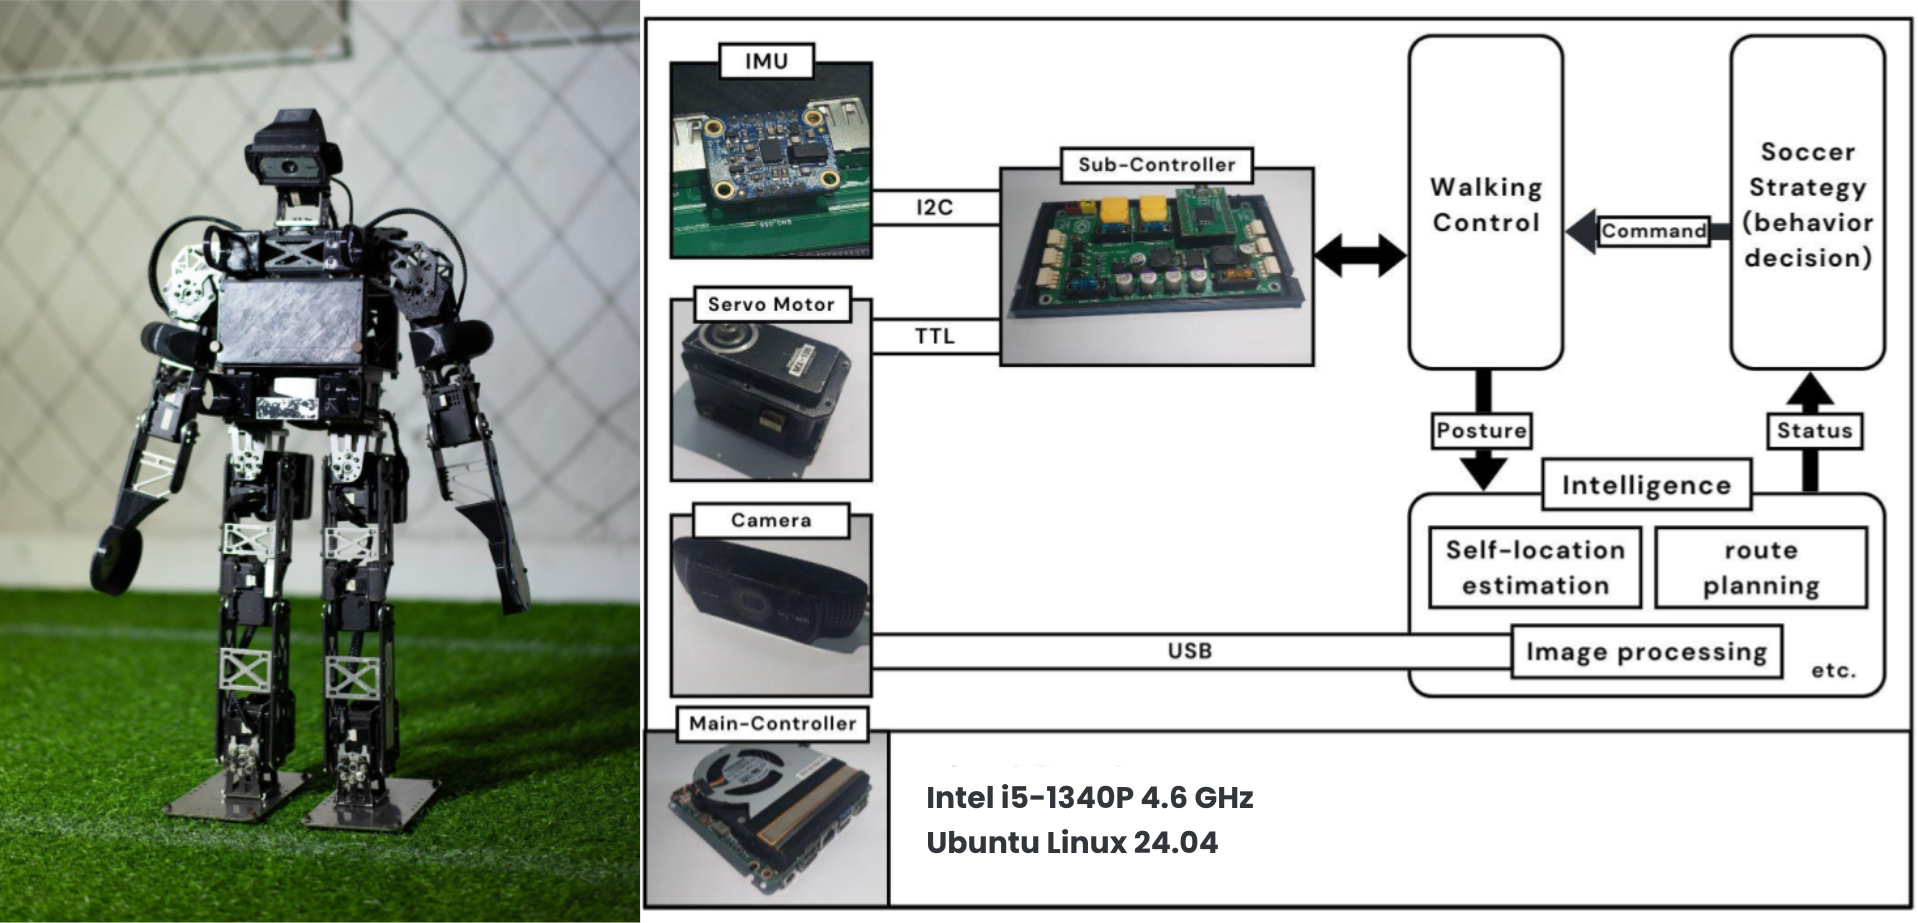
\includegraphics[width=\textwidth]{Ichiro Architecture.png}
\caption{ICHIRO ITS humanoid robot platform used in this research.}
\label{fig:ichiro}
\end{figure*}

\section{System Description} \label{sec:system_desc}

This section describes the humanoid robot platform and software framework used
in this research, providing the system context in which the proposed approach is implemented.

\subsection{ICHIRO ITS}

The system is implemented on humanoid soccer robots developed by the ICHIRO ITS
team from Sepuluh Nopember Institute of Technology. The team participates in humanoid
soccer competitions such as RoboCup, contributing to research and development
of humanoid robotics.



The robot is classified as a kid-size humanoid, equipped with 20 Degrees of Freedom (DOF)
driven by servo actuators. A monocular RGB camera (Logitech C930e) is mounted on the robot's
head and serves as the primary sensor for perception. Additional sensors include joint
encoders for all actuated joints and an Inertial Measurement Unit (IMU) that provides
orientation information. The robot runs on an Intel NUC i5 mini PC, while a custom control
module (CM) board is responsible for low-level sensor acquisition and actuator interfacing.
An overview of the robot platform is shown in Figure~\ref{fig:ichiro}.

\subsection{Robot Operating System 2}
The robot's software is built using the Robot Operating System 2 (ROS 2)
Jazzy Jalisco, which provides a modular, multi-process architecture.
The system uses the Data Distribution Service (DDS) middleware to
ensure robust inter-process communication with configurable Quality of Service
(QoS) policies. The ROS 2 framework facilitates a publisher-subscriber
model that allows independent nodes to share information through standardized
topics \cite{Macenski2022}.

In this research, the IPM implementation leverages existing software
modules: a Deep Neural Network (DNN) node that publishes detected objects
as bounding boxes, a joint state publisher that provides real-time servo
encoder values, and an IMU node that provides orientation feedback. These
synchronized data streams provide the necessary inputs for the IPM deprojection
algorithm, allowing the system to accurately correlate visual features in
image space with the robot's physical configuration in the real world.

\subsection{Universal Robot Description Format}

Universal Robot Description Format (URDF) is an XML-based format used to
model a robot's physical structure. This format is widely supported by
the robotics ecosystem, including ROS 2, and enables the construction of a
complete transformation tree. The transformations in this tree are constructed using
the ROS 2 \texttt{tf2} library and are broadcast by a publisher node,
allowing other nodes to consume synchronized pose data for real-time calculations.

The URDF for the ICHIRO ITS robot incorporates the 20 DOF servo actuators
along with a dedicated \texttt{camera\_frame}. This frame follows the
standard ROS vision axis convention where the $Z$-axis points forward
along the optical axis, the $Y$-axis points downward, and the $X$-axis
points to the right \cite{NVIDIA2026}. Additionally, the model
defines the \texttt{left\_foot\_frame} and \texttt{right\_foot\_frame},
which are used to dynamically compute the \texttt{base\_footprint}.
This virtual frame serves as the primary ground-level reference for
the \texttt{camera\_frame} in the IPM calculation, ensuring that visual
deprojections are correctly referenced to the playing surface.

\section{Theoretical Background} \label{sec:theories}

This section presents the theoretical foundations required for the
proposed approach, including camera projection models, kinematic transformations,
ground plane assumption, and the IPM formulation.

\subsection{Pinhole Camera Model}

The pinhole camera model describes the relationship between a three-dimensional
world point and the two-dimensional image plane, as shown in Equation~\ref{eq:pinhole}:

\begin{equation} \label{eq:pinhole}
\begin{split}
\begin{pmatrix} x \\ y \\ 1 \end{pmatrix} &=
\begin{bmatrix}
f_{x} & 0 & p_{x} & 0 \\
0 & f_{y} & p_{y} & 0 \\
0 & 0 & 1     & 0
\end{bmatrix}
\begin{bmatrix}
R & t \\
0 & 1 \\
\end{bmatrix}
\begin{pmatrix} X \\ Y \\ Z \\ 1 \end{pmatrix} \\
&= K \begin{bmatrix} R & t \\ 0 & 1 \end{bmatrix}
\begin{pmatrix} X \\ Y \\ Z \\ 1 \end{pmatrix}
\end{split}
\end{equation}
where:
\begin{itemize}
    \item $(x, y)$: Coordinates of the projected point on the 2D image plane.
    \item $(X, Y, Z)$: Coordinates of the point in the 3D world coordinate system.
    \item $K$: The camera intrinsic matrix, parameters unique to specific camera hardware,
               including the focal length $(f_x, f_y)$ and the principal point coordinates $(p_x, p_y)$.
    \item $R$: The camera rotation matrix $(3 \times 3)$, representing the orientation
               of the camera in the world frame.
    \item $t$: The camera translation vector $(3 \times 1)$, representing the position
               of the camera origin in the world frame.
\end{itemize}
This formulation follows the standard pinhole camera model widely used in computer
vision \cite{Hartley2003,Szeliski2011}.

\subsection{Kinematics Tree}
A kinematic tree represents the hierarchical relationship between rigid
bodies (links) connected by joints. In this structure, each node corresponds
to a specific coordinate frame, while the edges define the rigid transformations
between parent and child frames. This mathematical representation allows the pose
of any link or sensor within the tree to be computed relative to a global or local
reference frame through the use of chained homogeneous transformations \cite{Craig2009,Siciliano2010}.

A rigid body transformation between two frames is represented using
a $4 \times 4$ homogeneous transformation matrix as shown in Equation~\ref{eq:transformation_matrix}:
\begin{equation} \label{eq:transformation_matrix}
\mathbf{T}_{a}^{b} =
\begin{bmatrix}
\mathbf{R}_{a}^{b} & \mathbf{t}_{a}^{b} \\
\begin{matrix} 0 & 0 & 0 \end{matrix} & 1
\end{bmatrix}
\end{equation}
where $\mathbf{R}_{a}^{b}$ is a $3 \times 3$ rotation matrix and
$\mathbf{t}_{a}^{b}$ is a $3 \times 1$ translation vector from frame
$a$ to frame $b$. Using homogeneous transformation matrix, a point $P_a$ expressed
in coordinate frame $a$ is transformed into frame $b$ as shown in
Equation~\ref{eq:transformation_equation}:
\begin{equation} \label{eq:transformation_equation}
\begin{bmatrix} P_b \\ 1 \end{bmatrix} = \mathbf{T}_{a}^{b} \begin{bmatrix} P_a \\ 1 \end{bmatrix}
\end{equation}
This representation is commonly used in robotics to model body structures and
to compute forward kinematics \cite{Kajita2014}.

\subsection{Ground Plane Assumption}
Inverse Perspective Mapping relies on the assumption that objects of interest lie on a planar surface \cite{Mark2024}.
In humanoid soccer, this assumption is valid for objects such as the ball, goalposts, and field markings,
as the playing field is flat \cite{RoboCupHumanoidLeague2025}.

By constraining points to lie on a plane, we can recover the depth $Z_c$ along the optical axis
by defining a plane in the camera frame $P_c$ using the plane equation as shown in Equation~\ref{eq:plane_camera}:

\begin{equation} \label{eq:plane_camera}
n_c \cdot P_c + d = 0
\end{equation}
where $n_c = [n_x, n_y, n_z]^T$ is the plane normal in the camera frame and $d$
is the perpendicular distance from the camera origin to the plane \cite{Stewart2012}.

The normal $n_c$ can be derived by transforming the fixed ground normal from the \texttt{base\_footprint}
frame to the \texttt{camera\_frame}. Since the IPM algorithm assumes that all objects of interest
lie on a flat surface, the ground normal in the base frame is fixed as $n_b = [0, 0, 1]^T$.
By applying the rotation matrix $R_{c}^{b}$, we can express this
normal in the camera's coordinate system as shown in Equation~\ref{eq:base_plane_wrt_camera}

\begin{equation} \label{eq:base_plane_wrt_camera}
n_c = (R_{c}^{b})^{T} \cdot n_b = \begin{bmatrix} r_{31} \\ r_{32} \\ r_{33} \end{bmatrix}
\end{equation}
where $r_{31}, r_{32}, r_{33}$ represent the elements of the third row of the rotation matrix $R_{c}^{b}$.

\subsection{Inverse Perspective Mapping}
Inverse Perspective Mapping (IPM) aims to recover the three-dimensional
position of an image point under the assumption that it lies on a known
planar surface, typically the ground. Given the camera intrinsic parameters
and the camera pose relative to the ground, the depth of a projected image
point can be analytically recovered \cite{Bertozzi1998,Park2023}.

The pixel $(u, v)$ in the image plane can be converted to a three-dimensional coordinate in
the camera frame $P_c = [X_c, Y_c, Z_c]$ using the inverse pinhole camera model
from Equation~\ref{eq:pinhole}, which yields the relations in Equation~\ref{eq:coordinate_camera}:

\begin{equation} \label{eq:coordinate_camera}
\begin{bmatrix} X_c \\ Y_c \\ Z_c \end{bmatrix} = Z_c 
\begin{bmatrix} \frac{u - p_x}{f_x} \\ \frac{v - p_y}{f_y} \\ 1 \end{bmatrix} = Z_c 
\begin{bmatrix} x \\ y \\ 1 \end{bmatrix}
\end{equation}
where $(x, y)$ are normalized image coordinates.

By substituting $P_c = [x Z_c, y Z_c, Z_c]^T$ into Equation~\ref{eq:plane_camera}, with
the distance $d$ from the plane in the \texttt{camera\_frame} equal to
the camera translation $t_z$ along the vertical axis relative to the base frame,
the value of $Z_c$ can be calculated as shown in Equation~\ref{eq:zc}:

\begin{equation} \label{eq:zc}
Z_c = \frac{-t_z}{r_{31} x + r_{32} y + r_{33}}
\end{equation}

Once $P_c$ is fully determined, the estimated position relative to the robot $P_b$
is obtained by transforming $P_c$ into the \texttt{base\_footprint} frame via the 
coordinate mapping in Equation~\ref{eq:pb_final}:

\begin{equation} \label{eq:pb_final}
\begin{bmatrix} P_b \\ 1 \end{bmatrix} = \mathbf{T}_{c}^{b} \begin{bmatrix} P_c \\ 1 \end{bmatrix}
\end{equation}
where $\mathbf{T}_{c}^{b}$ is the $4 \times 4$ homogeneous transformation matrix.
The system rejects any results where $Z_c \leq 0$ or is undefined (NaN),
as these indicate points behind the camera or parallel to the optical axis.

\section{Methodology}

This section focuses on practical aspects, including camera calibration,
robot kinematic frame construction, and the integration of the IPM module for object distance estimation.

\subsection{Camera Calibration}
The objective of camera calibration is to obtain the intrinsic parameters ($K$)
required for the projection calculation between the three-dimensional world and two-dimensional
image plane, as described in Equation~\ref{eq:pinhole}. In this paper, we used a Logitech C930e camera mounted
on the robot's head.

The calibration was conducted using a standard $8 \times 6$ checkerboard with known
square dimensions. We captured approximately 15 images of the checkerboard from
various distances and angles as shown in Figure~\ref{fig:camera_calib}.

\begin{figure}[!h]
\centering
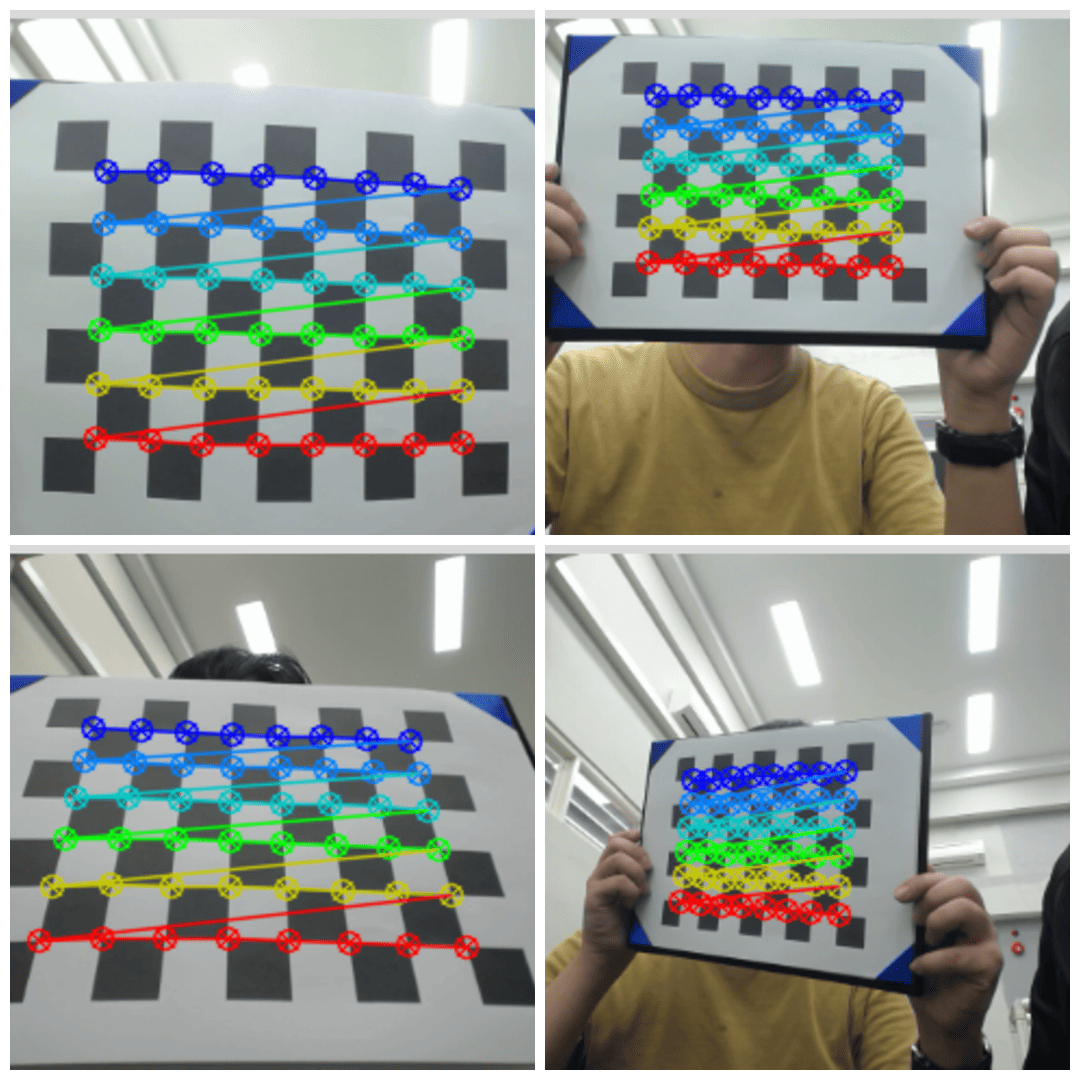
\includegraphics[width=0.72\columnwidth]{camera-calibration.png}
\caption{Visualization of detected checkerboard corners used for camera calibration.}
\label{fig:camera_calib}
\end{figure}

These images were then processed using the OpenCV
calibration library to estimate the focal length $(f_x, f_y)$ and principal point
coordinates $(p_x, p_y)$. While the calibration script also calculates lens distortion coefficients, the
radial and tangential distortion values for the Logitech C930e were found to be
sufficiently small to be neglected.

\subsection{Robot Frames Package}
In this research, we implemented a dedicated ROS 2 package, \texttt{robot\_frames},
which loads the URDF model and broadcasts kinematic transformations using the \texttt{tf2} library.
By consuming live joint encoder and IMU data, the package provides real-time kinematic transformations
that reflect the robot's physical state in the real world.

In addition, the package computes the \texttt{base\_footprint}, a virtual frame that serves as the
reference frame for IPM calculations. This frame is calculated dynamically using information from
the \texttt{right\_foot\_frame} and \texttt{left\_foot\_frame}. Since the robot is always in contact
with the ground, the $Z$-height of the \texttt{base\_footprint} is set to match the supporting foot
(i.e., the foot currently in contact with the ground). Meanwhile, the $X$ and $Y$ coordinates are
defined as the midpoint between both feet.

The overall procedure of the robot frame computation is summarized
in Algorithm~\ref{alg:robot_frames}.

\begin{algorithm}[!h]
\caption{Robot Frames Package}
\label{alg:robot_frames}
\footnotesize
\begin{algorithmic}[1]
\Require URDF path $(f)$
\Ensure TF frames $(\mathcal{T})$

\State $R \gets \text{ParseURDF}(f)$
\State $J \gets \text{ExtractJoints}(R)$

\While{running}
    \State $q \gets \text{ReadJointEncoders}()$
    \State $(r,p,\psi) \gets \text{ReadIMU}()$
    \State $(x,y) \gets \text{ReadOdometry}()$

    \State $\text{UpdateState}(q, r,p,\psi, x,y)$
    \State $\mathcal{T} \gets \emptyset$

    \ForAll{$j \in J$}
        \State $F \gets \text{ComputeTransform}(j)$
        \If{$j = \text{"body\_joint"}$}
            \State $F \gets \text{ApplyIMU}(F, r,p,\psi, x,y)$
        \EndIf
        \State $\mathcal{T} \gets \mathcal{T} \cup \{F\}$
    \EndFor

    \State $B \gets \text{ComputeBaseFootprint}()$
    \State $\mathcal{T} \gets \mathcal{T} \cup \{B\}$

    \State $\text{BroadcastTF}(\mathcal{T})$
\EndWhile

\end{algorithmic}
\end{algorithm}

\subsection{IPM Package}

We implemented another dedicated ROS~2 package, \texttt{ipm}, to perform distance estimation using
the Inverse Perspective Mapping (IPM) algorithm. This package subscribes to object bounding boxes
produced by a Deep Neural Network (DNN) detection module and kinematic transformations provided by
the \texttt{robot\_frames} package. In addition, it loads a JSON configuration file containing the
camera intrinsic parameters ($K$) obtained from the calibration process.

For each detected object, a representative image pixel $(x, y)$ is selected to approximate the
object's contact point with the ground. For objects such as other robots or goalposts, the
bottom-center of the bounding box is selected. For objects such as the ball or field markers,
the center of the bounding box is used.

Note that for certain objects, such as the ball, the selected pixel may not correspond to direct
ground contact. This discrepancy is handled by introducing a height offset ($h$), which effectively
treats the ground plane as being elevated by that amount. Since the physical dimensions of the ball
are known, the height offset $h$ corresponds to its radius. Consequently, the depth recovery
equation defined in Equation~\ref{eq:zc} is modified as shown in Equation~\ref{eq:zc_final}:

\begin{equation} \label{eq:zc_final}
Z_c = \frac{h - t_z}{r_{31}x + r_{32}y + r_{33}}
\end{equation}

The complete IPM projection pipeline is described in
Algorithm~\ref{alg:ipm}.

\begin{algorithm}[!h]
\caption{IPM Package}
\label{alg:ipm}
\footnotesize
\begin{algorithmic}[1]
\Require TF Frames ($\mathcal{T}$)
\Ensure Projected Object Positions ($\mathcal{P}$)

\State $K \gets \text{LoadCameraIntrinsics}()$
\While{receiving detections}
    \State $\mathcal{O} \gets \text{ReadDetections}()$
    \State $\mathcal{P} \gets \emptyset$
    \State $(R, t) \gets \text{LookupTransform}(\mathcal{T}, \text{camera} \rightarrow \text{base\_footprint})$

    \ForAll{$o \in \mathcal{O}$}
        \State $u \gets (o.left + o.right)/2$
        \If{$o.\text{label} \in \{\text{"robot"}, \text{"goalpost"}\}$}
            \State $v \gets o.bottom$
        \Else
            \State $v \gets (o.top + o.bottom)/2$
        \EndIf

        \State $(x, y) \gets \text{NormalizePixel(u, v, K)}$

        \State $h \gets 0$
        \If{$o.\text{label} = \text{"ball"}$}
            \State $h \gets \text{ball radius}$
        \EndIf

        \State $Z_c \gets \dfrac{h - t_z}{r_{31}x + r_{32}y + r_{33}}$
        \If{$Z_c \leq 0$}
            \State \textbf{continue}
        \EndIf

        \State $P_c \gets (Z_c \cdot x, Z_c \cdot y, Z_c)$
        \State $P_b \gets R \cdot P_c + t$

        \State $\mathcal{P} \gets \mathcal{P} \cup \{P_w\}$

    \EndFor

    \State $\text{Publish}(\mathcal{P})$
\EndWhile

\end{algorithmic}
\end{algorithm}

\section{Evaluation}

This section evaluates the proposed IPM distance estimation under static
and dynamic walking conditions using identical object configurations to ensure
consistency. The static evaluation measures estimation accuracy when the robot remains
stationary, while the dynamic evaluation analyzes performance during
walking, where object positions are expressed in global coordinates
using odometry. A comparison with the previously used regression-based
method is also conducted to demonstrate the advantages of the proposed
approach across varying distances.

\subsection{Experimental Setup}

All experiments were conducted on a $6 \times 9$ m kid-size field
following the RoboCup 2026 rules.
The robot is initialized at the same global position for both
static and dynamic evaluations, namely the kickoff position
$P(450.0, 300.0)$ at the center of the field.

A fixed set of objects is placed at known global coordinates
and remains unchanged throughout all trials.
Each object is assigned a symbolic notation for concise reference
in subsequent tables and equations.

\begin{table}[h]
\centering
\caption{Fixed object configuration used in all experiments}
\label{tab:object_setup}
\begin{tabular}{c c c}
\hline
Symbol & Object & Global Position $(X_i, Y_i)$ [cm] \\
\hline
$O_1$ & Soccer Ball & $(550.0, 350.0)$ \\
$O_2$ & Opponent Robot & $(650.0, 200.0)$ \\
$O_3$ & X-Intersection & $(750.0, 300.0)$ \\
$O_4$ & L-Intersection & $(800.0, 450.0)$ \\
$O_5$ & T-Intersection & $(900.0, 450.0)$ \\
$O_6$ & Left Goalpost & $(900.0, 190.0)$ \\
\hline
\end{tabular}
\end{table}

The global coordinates $(X_i, Y_i)$ are determined using field geometry
and manual measurement to ensure repeatability. These positions remain
constant for both static and dynamic experiments. The complete experimental
configuration deployed on the RoboCup field is presented in
Figure~\ref{fig:combined_setup}, which illustrates the schematic target layout
(a) alongside the physical test platform deployment (b).

\begin{figure*}[!h]
\centering
\begin{minipage}[b]{0.6\textwidth}
\centering
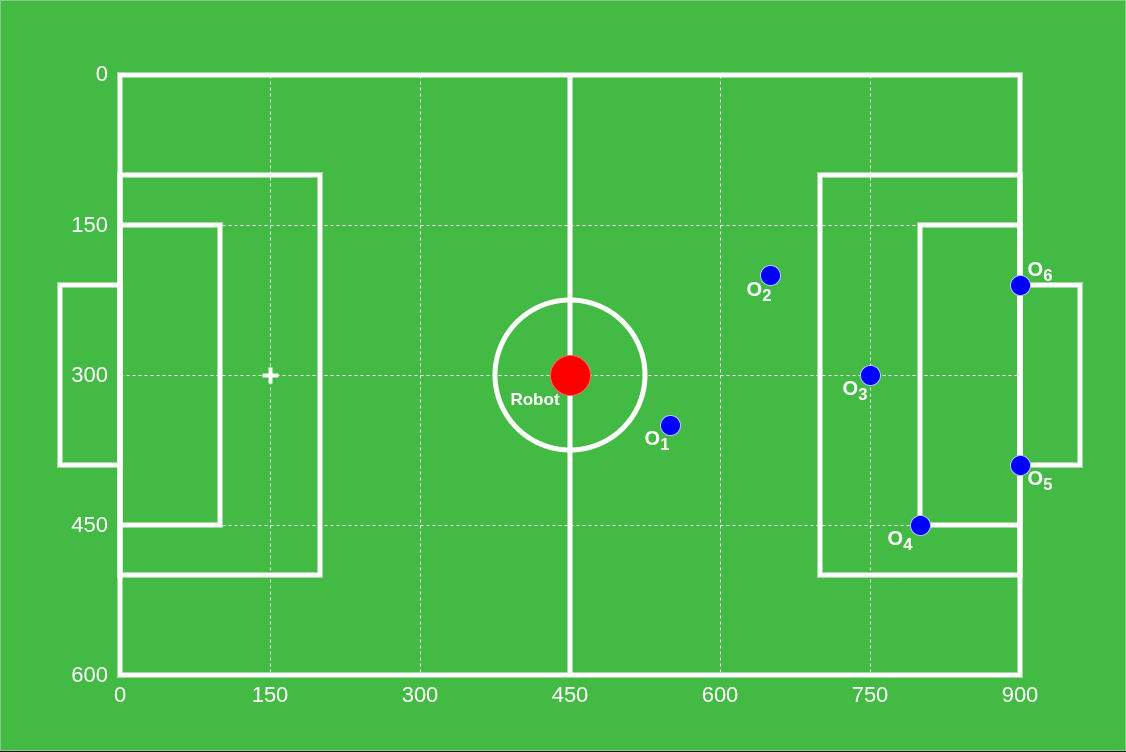
\includegraphics[width=\textwidth]{Experiment Setup.png}
\\ \vspace{1mm} \footnotesize (a) Schematic diagram of target configurations.
\end{minipage}
\hfill
\begin{minipage}[b]{0.36\textwidth}
\centering
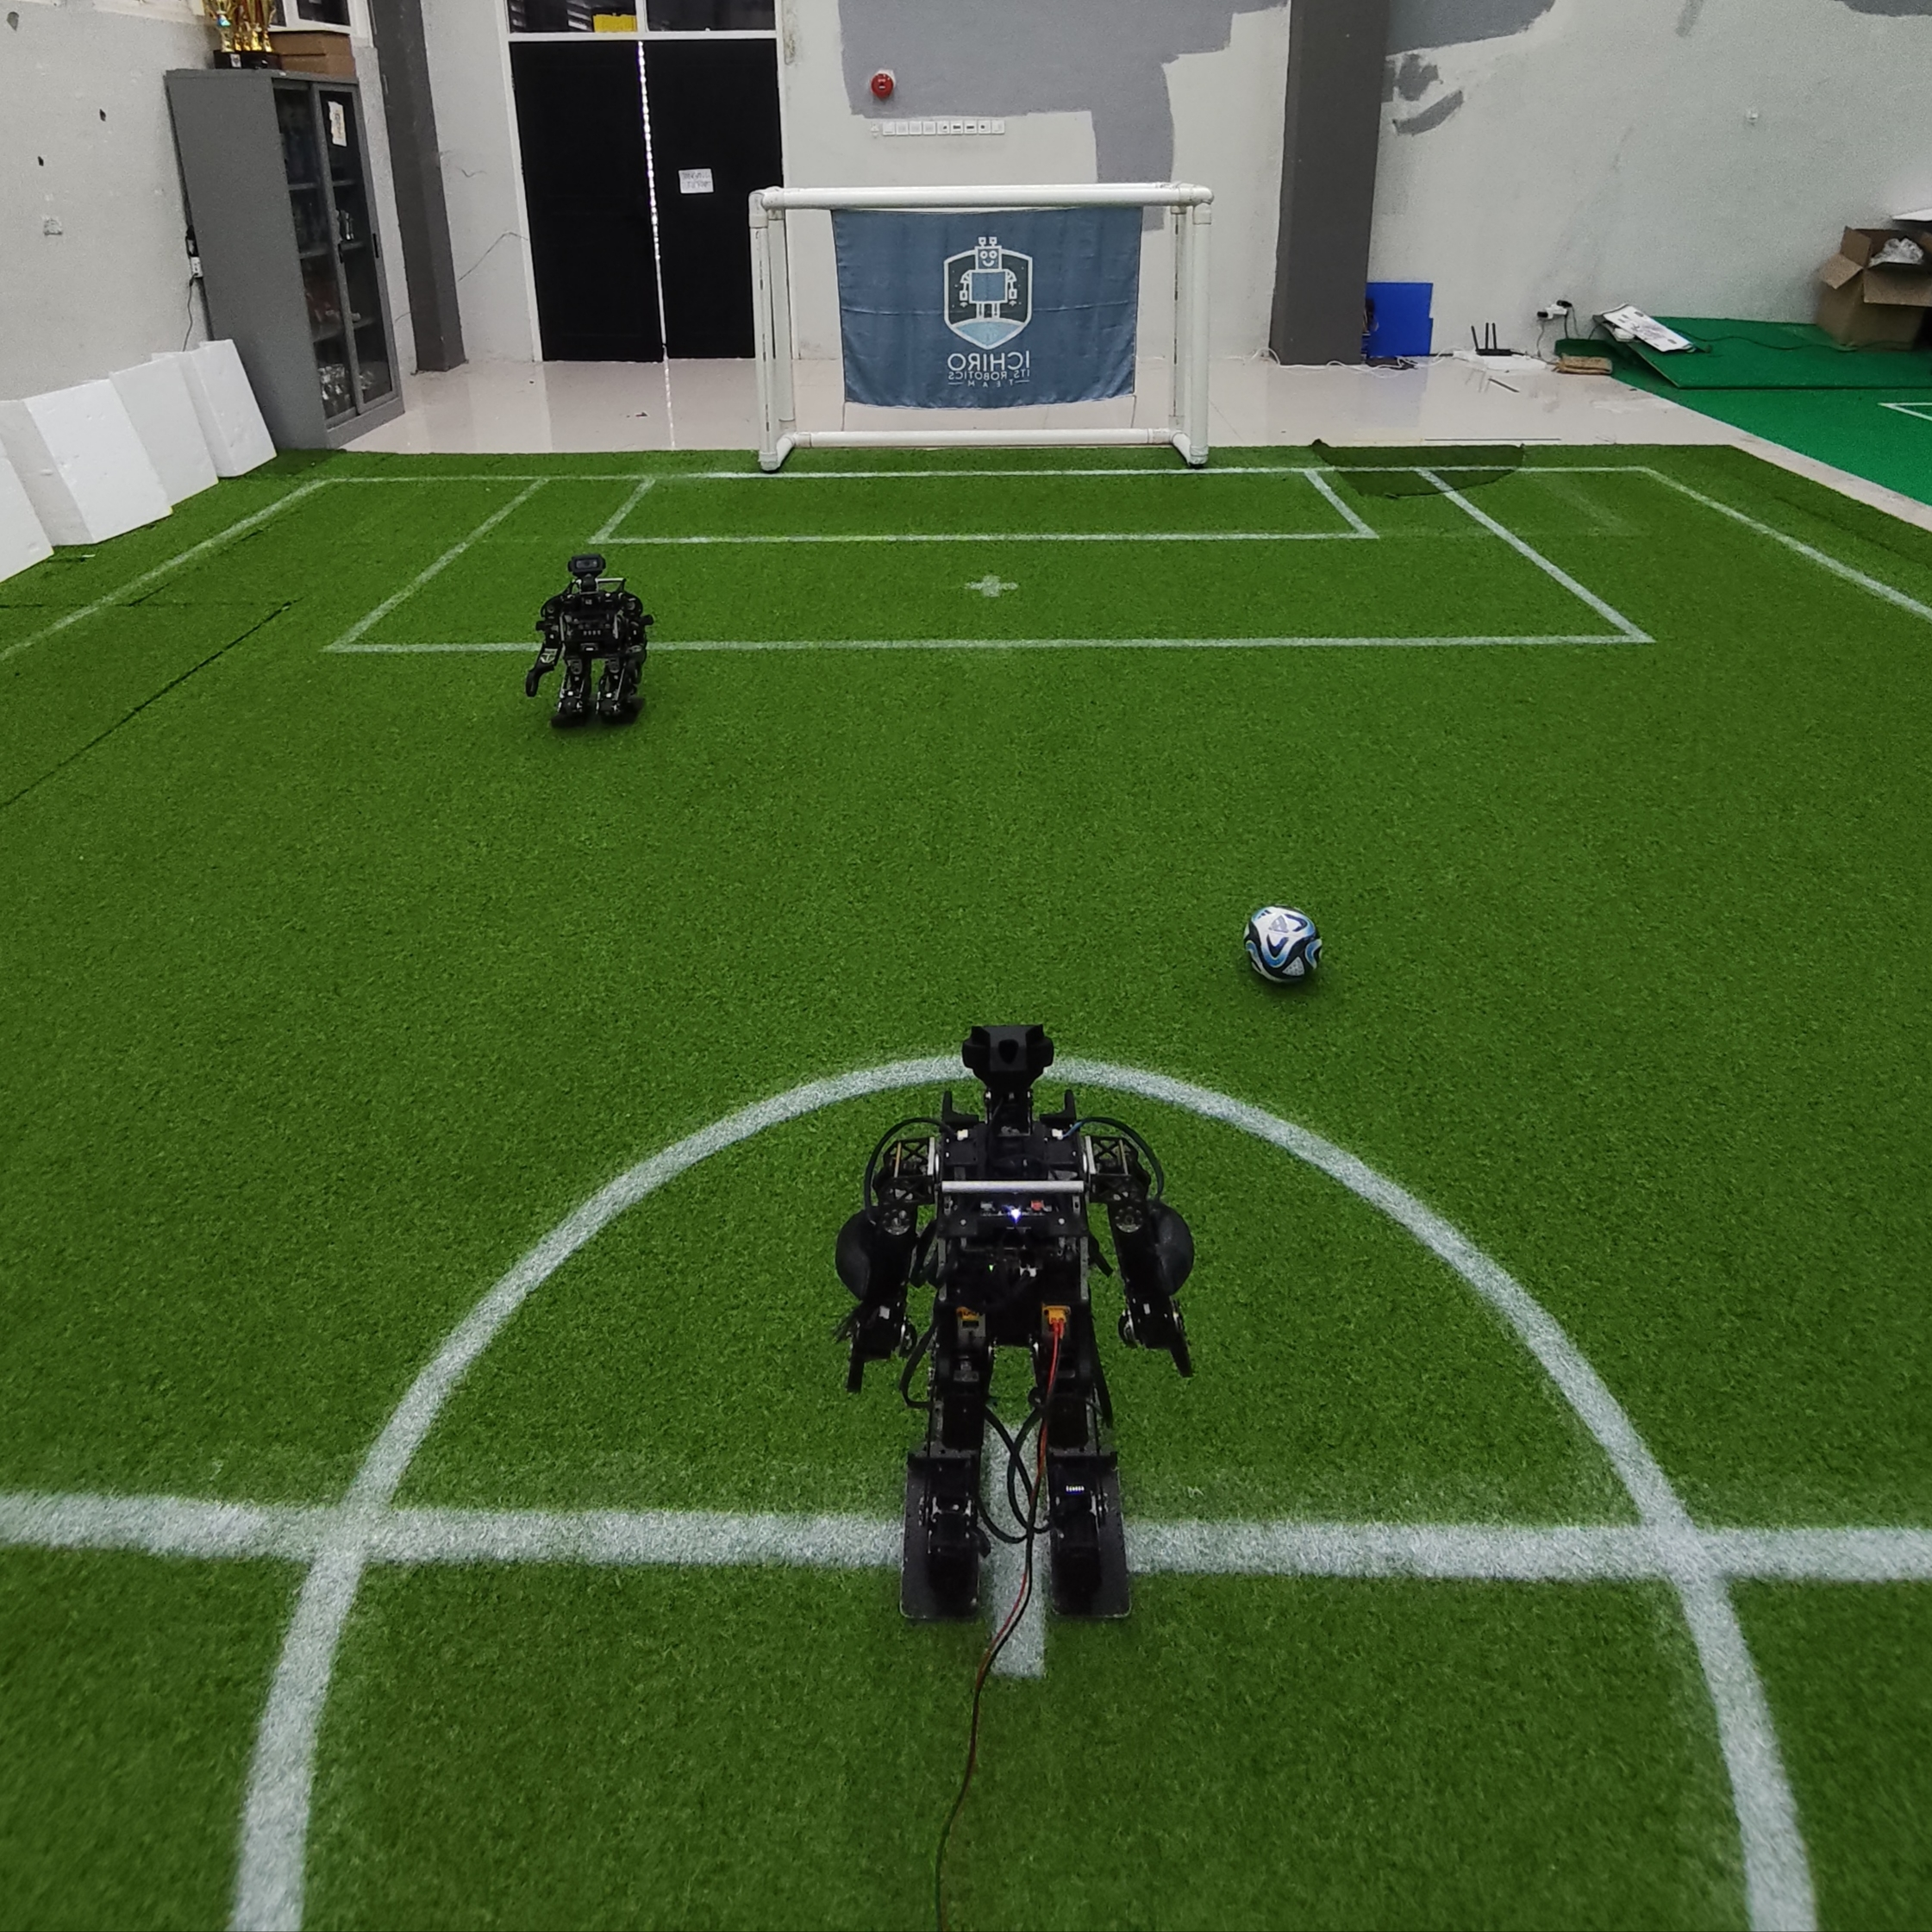
\includegraphics[width=\textwidth]{Real Setup.jpg}
\\ \vspace{1mm} \footnotesize (b) Physical test platform deployment.
\end{minipage}
\caption{Complete experimental configuration deployed on the RoboCup field, displaying
the robot starting kickoff orientation and the fixed global coordinates for
targets $O_1$--$O_6$.}
\label{fig:combined_setup}
\end{figure*}

To assess the precision of the IPM estimations, the estimated target coordinates
$(\hat{X}, \hat{Y})$ are compared with ground-truth positions $(X, Y)$. Axis-wise errors
are defined as $E_x = \hat{X} - X$ and $E_y = \hat{Y} - Y$, yielding the aggregate
Euclidean position error as defined in Equation~\ref{eq:euclidean_error}:

\begin{equation} \label{eq:euclidean_error}
E = \sqrt{(E_x )^2 + ( E_y )^2}
\end{equation} 

All metrics are expressed in centimeters (cm). The distribution of tracking errors
is summarized using Mean Absolute Error (MAE), Root Mean Square Error (RMSE), median error,
Median Absolute Deviation (MAD), and standard deviation ($\sigma$). To establish
statistical significance, 95\% confidence intervals are estimated via bootstrap resampling
with 10,000 iterations.

\subsection{Static Evaluation}

In the static evaluation, the robot remains stationary at the kickoff
position $P(450.0, 300.0)$, and both the body and head are kept fixed.
Since the robot pose is known and constant, it is used as the reference
pose for transforming the estimated object positions into the global
field coordinate system.

For each object, the IPM module estimates the relative position
$(X_b, Y_b)$ with respect to the \texttt{base\_footprint} frame.
The estimated global position $(\hat{X}_i, \hat{Y}_i)$ is obtained
by applying a rigid body transformation using the known robot pose as
shown in Equation~\ref{eq:global_transform}:

\begin{equation} \label{eq:global_transform}
\begin{bmatrix}
\hat{X}_i \\
\hat{Y}_i \\
1
\end{bmatrix}
=
\mathbf{T}_{b}^{g}
\begin{bmatrix}
X_b \\
Y_b \\
1
\end{bmatrix}
\end{equation}
where $\mathbf{T}_{b}^{g}$ denotes the homogeneous transformation
from the \texttt{base\_footprint} frame to the global field frame.

For each object, Euclidean errors were computed for every frame in the
recorded image sequence while the robot and objects remained stationary.
Table~\ref{tab:static_results} summarizes the corresponding error statistics.

\begin{table}[h]
\centering
\footnotesize
\caption{Static IPM estimation error statistics}
\label{tab:static_results}
\begin{tabular}{c c c c c c}
\toprule
\textbf{Obj.} &
\textbf{MAE} &
\textbf{RMSE} &
\textbf{Median} &
\textbf{MAD} &
\textbf{$\sigma$} \\
\midrule
$O_1$ & 1.61 & 1.62 & 1.78 & 0.17 & 0.19 \\
$O_2$ & 6.61 & 6.62 & 6.74 & 0.13 & 0.40 \\
$O_3$ & 3.33 & 3.33 & 3.33 & 0.00 & 0.00 \\
$O_4$ & 7.05 & 7.05 & 7.08 & 0.03 & 0.10 \\
$O_5$ & 21.30 & 22.16 & 18.63 & 3.50 & 6.11 \\
$O_6$ & 38.80 & 38.80 & 38.80 & 0.00 & 0.00 \\
\bottomrule
\end{tabular}
\end{table}

The results indicate that the proposed IPM method achieves high positional
accuracy for nearby and intermediate-distance objects. Objects $O_1$--$O_4$
exhibit MAE values below 8~cm and standard deviations below 0.5~cm, indicating
both accurate and stable estimations under static conditions.

Among the evaluated objects, $O_1$ achieves the lowest error with an MAE of
1.61~cm, while $O_6$ exhibits the largest error with
an MAE and RMSE of 38.80~cm. The results show a clear increase in estimation
error as object distance from the robot increases, particularly for the
distant targets $O_5$ and $O_6$.

This behavior is inherent to monocular IPM-based depth estimation.
With the robot head maintained at a tilt angle of $0^\circ$, objects located
farther from the robot project closer to the image horizon due to perspective
effects. In this region, small variations in image coordinates correspond to
large variations in the estimated depth. Consequently, the depth term computed
in Equation~\ref{eq:zc_final} becomes increasingly sensitive to joint offsets,
detection inaccuracies, and calibration errors, resulting in larger
estimation deviations for distant objects.

Figure~\ref{fig:static_ipm_evaluation} visualizes the mean estimated positions and
corresponding error vectors in field coordinates. The estimated positions remain
close to their respective ground-truth locations for nearby objects, while the
magnitude of the error vectors increases for distant targets.

\begin{figure}[h]
\centering
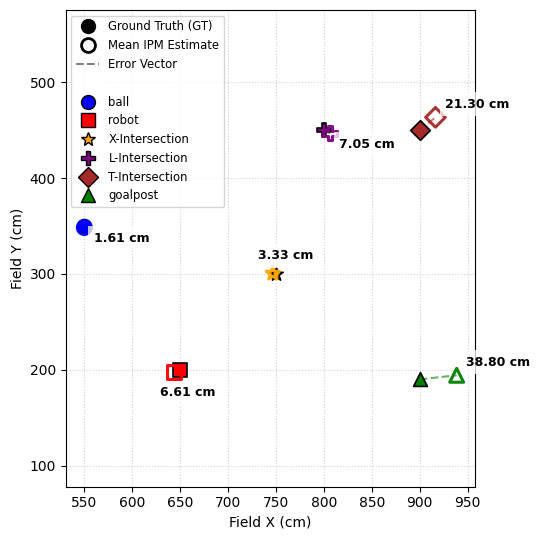
\includegraphics[width=\columnwidth]{static_ipm_evaluation_2.png}
\caption{Static IPM evaluation in field coordinates, showing reference
positions, mean IPM estimates, and error vectors for all evaluated objects.}
\label{fig:static_ipm_evaluation}
\end{figure}

In addition, $O_5$ exhibits the highest variance among all evaluated objects,
with a standard deviation of 6.11~cm and a wider margin of uncertainty
(MAE 95\% CI: [19.04, 24.12]). This behavior is attributed to small variations
in the detected bounding-box center across frames. Although the object is
consistently detected, slight changes in the predicted bounding box lead to
different IPM estimates. Because the effect is amplified for distant objects,
the resulting position estimates exhibit higher variance other evaluated targets.

\begin{figure}[h]
  \centering
  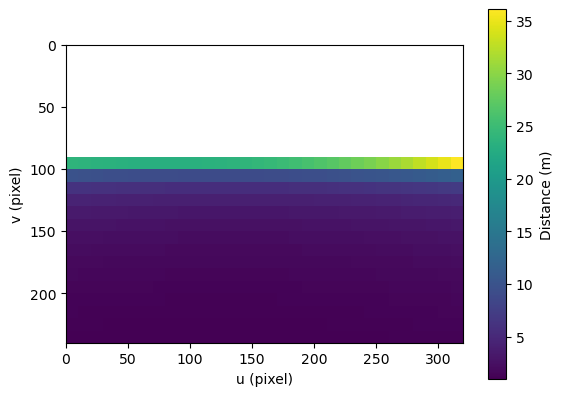
\includegraphics[width=0.48\textwidth]{ipm_distances.png}
  \caption{Numerical simulation of IPM distance mapping from a $32 \times 24$ pixel grid, showing exponential depth sensitivity and the invalid region above the horizon.}
  \label{fig:ipm_numerical_simulation}
\end{figure}

To further validate these experimental observations, a theoretical numerical 
simulation was conducted. A downsampled $32 \times 24$ pixel grid was passed 
through the IPM model to isolate the geometric behavior of the projection without 
physical sensor noise. As illustrated in Figure~\ref{fig:ipm_numerical_simulation},
the mapping from image coordinates $(u, v)$ to field distance is highly non-linear. 
At the lower regions of the image (close targets), a one-pixel shift represents a 
negligible change in distance. However, as the coordinates approach the horizon line, 
the step size per pixel increases exponentially, and any projection above the horizon 
becomes completely invalid. This simulation structurally confirms why both the systematic 
errors ($O_6$) and the frame-to-frame variance ($O_5$) escalate dramatically with distance.


% \newpage

\subsection{Dynamic Evaluation}

The dynamic evaluation extends the experiment to conditions in
which the robot is walking. The robot starts from the same kickoff
position $P(450.0, 300.0)$ and walks forward for 1 meter toward target point
$P'(550.0, 300.0)$, repeated for 10 trials.

During walking, the robot head performs continuous scanning motions
to detect visible objects. The IPM module continuously estimates
the relative object positions $(X_b, Y_b)$ in the
\texttt{base\_footprint} frame.

To express object positions in global coordinates, the relative
IPM outputs are transformed using the robot pose estimated from odometry
via the relationship in Equation~\ref{eq:odom_transform}:

\begin{equation} \label{eq:odom_transform}
\begin{bmatrix}
\hat{X}_i \\
\hat{Y}_i \\
1
\end{bmatrix}
=
\mathbf{T}_{b,\text{odom}}^{g}
\begin{bmatrix}
X_b \\
Y_b \\
1
\end{bmatrix}
\end{equation}

Certain objects are excluded from the dynamic evaluation. In particular,
the L-intersection ($O_4$) and T-intersection ($O_5$) are not considered,
as multiple instances of these features are detected at different
locations during walking. Additionally, the goalpost ($O_6$) is excluded because of
ambiguity when only a single post, rather than the complete goal, is detected.
This ambiguity makes it difficult to associate detections with a unique reference position.
Therefore, only objects with consistent and unambiguous detections are included in the analysis.

\begin{table}[h]
\centering
\footnotesize
\caption{Dynamic IPM estimation results (10 trials)}
\label{tab:dynamic_results}
\begin{tabular}{c c c c c c}
\toprule
\textbf{Obj.} &
\textbf{MAE} &
\textbf{RMSE} &
\textbf{Median} &
\textbf{MAD} &
\textbf{$\sigma$} \\
\midrule
$O_1$ & 32.08 & 62.81  & 12.74 & 25.33 & 54.00  \\
$O_2$ & 62.16 & 113.87 & 14.75 & 55.05 & 95.41  \\
$O_3$ & 61.05 & 123.33 & 5.11  & 58.74 & 107.16 \\
\bottomrule
\end{tabular}
\end{table}

Table~\ref{tab:dynamic_results} presents the aggregated dynamic evaluation
results. Compared with the static evaluation, all objects exhibit substantially
larger MAE, RMSE, and standard deviation values. This increase is expected because
the robot continuously performs locomotion and head scanning motions, introducing
additional uncertainty in object detection, camera pose estimation, and odometry error.

Despite the increase in aggregate error metrics, the median error remains
relatively low for all evaluated objects. The median errors are
12.74~cm (95\% CI: 11.83--13.55~cm), 14.75~cm (95\% CI: 12.10--17.46~cm),
and 5.11~cm (95\% CI: 3.70--8.55~cm) for $O_1$, $O_2$, and $O_3$,
respectively. The relatively narrow confidence intervals indicate that
the typical estimation error remains consistently small across repeated
trials. This suggests that most position estimates remain close to the
corresponding reference positions during walking.

\begin{table}[!h]
\centering
\footnotesize
\caption{Shapiro--Wilk test results for dynamic evaluation errors}
\label{shapiro_wilk_test}
\begin{tabular}{lcc}
\toprule
\textbf{Object} & \textbf{Statistic} & \textbf{p-value} \\
\midrule
$O_1$ & 0.5424 & $6.05 \times 10^{-26}$ \\
$O_2$ & 0.6558 & $4.53 \times 10^{-23}$ \\
$O_3$ & 0.5756 & $8.17 \times 10^{-21}$ \\
\bottomrule
\end{tabular}
\end{table}

However, the substantial gap between the median and RMSE values suggests
that the error distribution is highly asymmetric. A small number of
large estimation failures significantly increase the mean-based metrics,
while the majority of observations remain concentrated near the true
object locations.

To assess the normality of the dynamic error distributions, the
Shapiro--Wilk test was performed for each evaluated object. As shown in
Table~\ref{shapiro_wilk_test}, all objects produce extremely small
p-values ($p < 0.05$), rejecting the null hypothesis of normally
distributed errors. Consistent with this result, the Q--Q plots in
Figure~\ref{fig:dynamic_qq_plots} exhibit pronounced upward curvature
at the upper quantiles, indicating heavily right-skewed distributions
caused by occasional large estimation failures. Consequently, robust
statistics such as the median and MAD provide a more representative
description of typical system performance than mean-based metrics alone.

\begin{figure*}[h]
\centering
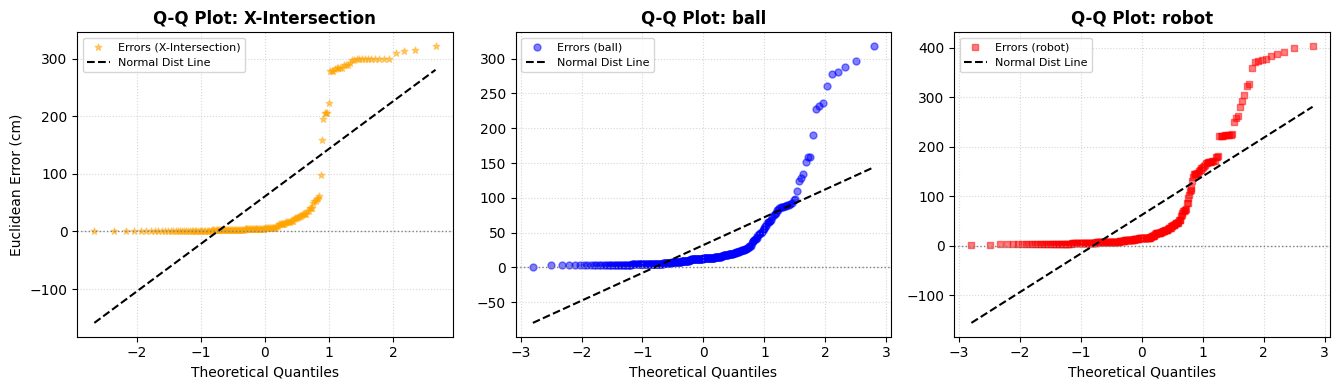
\includegraphics[width=\textwidth]{dynamic_errors_qq_plots.png}
\caption{Quantile-Quantile (Q-Q) plots of Euclidean distance errors for
the ball ($O_1$), robot ($O_2$), and X-intersection ($O_3$) during dynamic
walking trials. The sharp upward curve away from the straight normal
line shows that the errors do not follow a normal distribution, but are heavily
right-skewed due to occasional large estimation spikes.}
\label{fig:dynamic_qq_plots}
\end{figure*}

The spatial distribution of the estimates is shown in
Figure~\ref{fig:dynamic_ipm_evaluation}. A 15~cm tolerance circle is
drawn around each reference object position. Using this threshold,
the proposed method achieves successful position estimation rates of
59.5\%, 50.2\%, and 62.2\% for objects $O_1$, $O_2$, and $O_3$,
respectively. These results indicate that a majority of object position
estimates remain within 15~cm of the reference position despite the
robot being in motion.

\begin{figure*}[t]
\centering
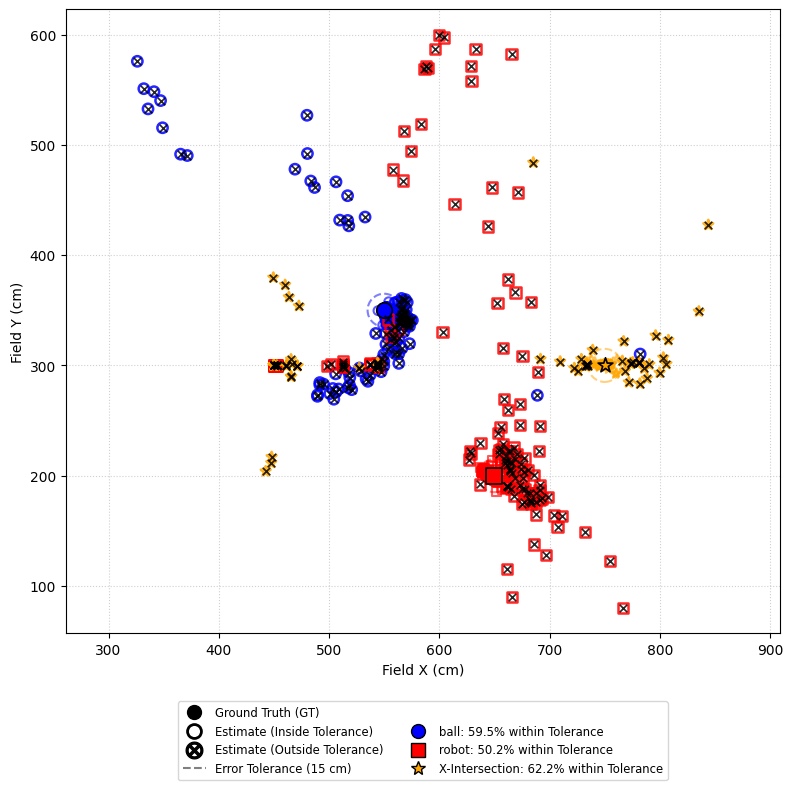
\includegraphics[width=0.7\textwidth]{dynamic_ipm_evaluation_2.png}
\caption{Dynamic IPM evaluation in field coordinates during active walking,
displaying spatial distribution arrays, true reference markers, and the
designated 15~cm error tolerance boundaries for targets $O_1$, $O_2$, and $O_3$.}
\label{fig:dynamic_ipm_evaluation}
\end{figure*}

Several failure cases were observed in which estimated object positions
were projected to unrealistic field locations. Because IPM derives
world coordinates directly from image measurements, small errors in
object detection, camera pose, or calibration can be amplified into
large position errors, particularly for distant objects near the image
horizon.

It is important to note that odometry is not involved in the IPM
distance computation itself. IPM estimates object positions purely
relative to the robot. Odometry is only used to express estimated
object positions in global coordinates during dynamic evaluation.
Therefore, the measured dynamic error is influenced by both IPM
estimation error and odometry drift. To better understand this
influence, odometry error is analyzed independently using the
approach proposed by Martinelli~\cite{Martinelli2001APS}.

The method characterizes odometry uncertainty using four parameters:
translational bias ($E_t$), translational noise ($K_\rho$),
rotational bias ($E_r$), and rotational noise ($K_\theta$).
The bias terms represent systematic errors, while the noise terms
capture random variations caused by sensor noise and surface interaction.

The odometry error parameters estimated at the target position $P'(550.0, 300.0)$ are: 
$E_r = 0.0005$ deg/cm, $K_\theta = 0.1994$ deg$^2$/cm, $E_t = -1.6902\%$, and $K_\rho = 0.042551$~cm. 
These values indicate that both systematic and non-systematic errors remain 
relatively small over the 1~m walking trajectory. Specifically, the low 
rotational bias ($E_r$) and minor translational bias ($E_t$) confirm that the 
robot maintains a consistent heading and expected traveled distance. 

% \newpage

\begin{figure*}[!h]
\centering
\begin{minipage}[b]{0.48\textwidth}
\centering
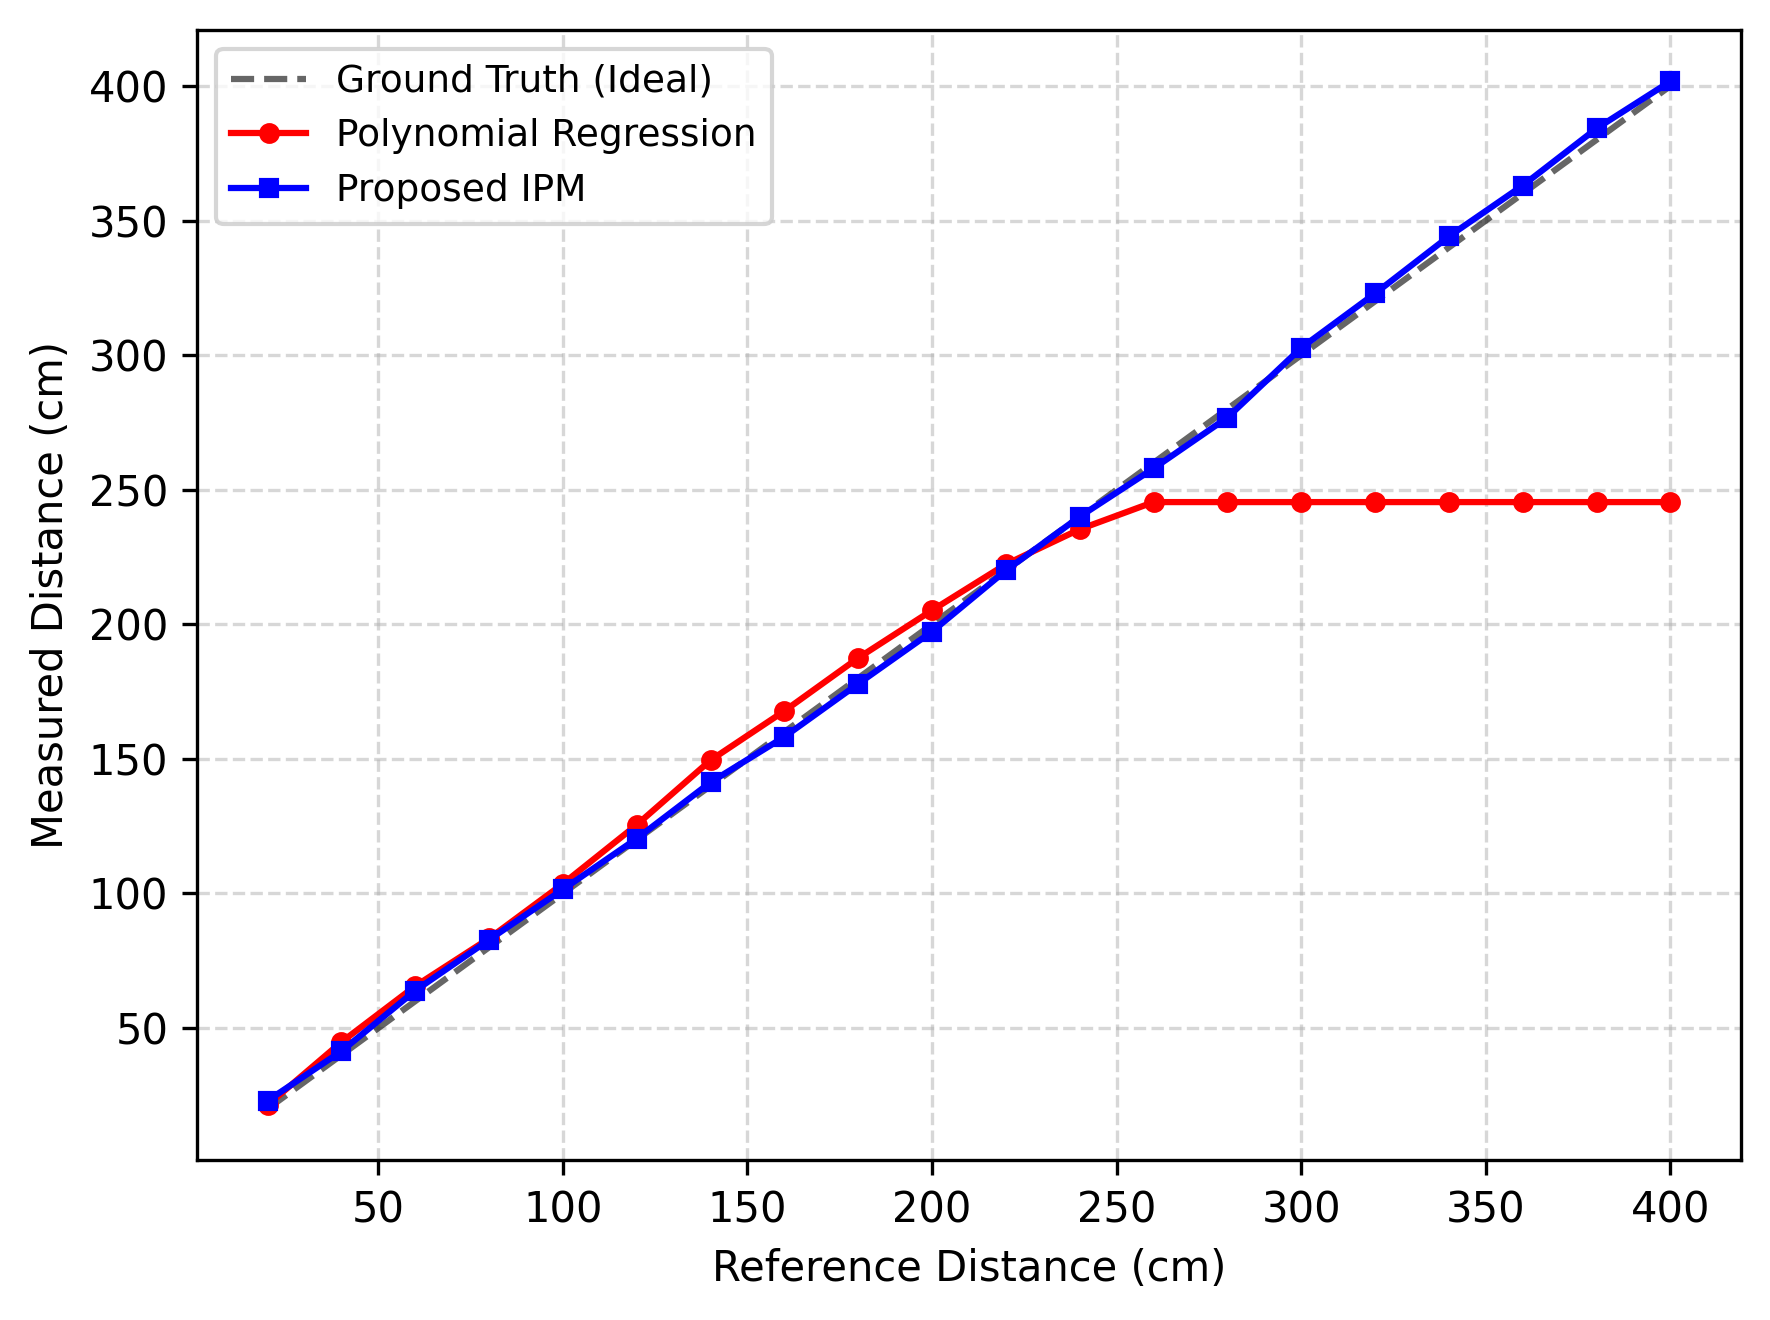
\includegraphics[width=\textwidth]{regression_vs_ipm_estimates.png}
\\ \vspace{1mm} \footnotesize (a) Distance estimates comparison.
\end{minipage}
\hfill
\begin{minipage}[b]{0.48\textwidth}
\centering
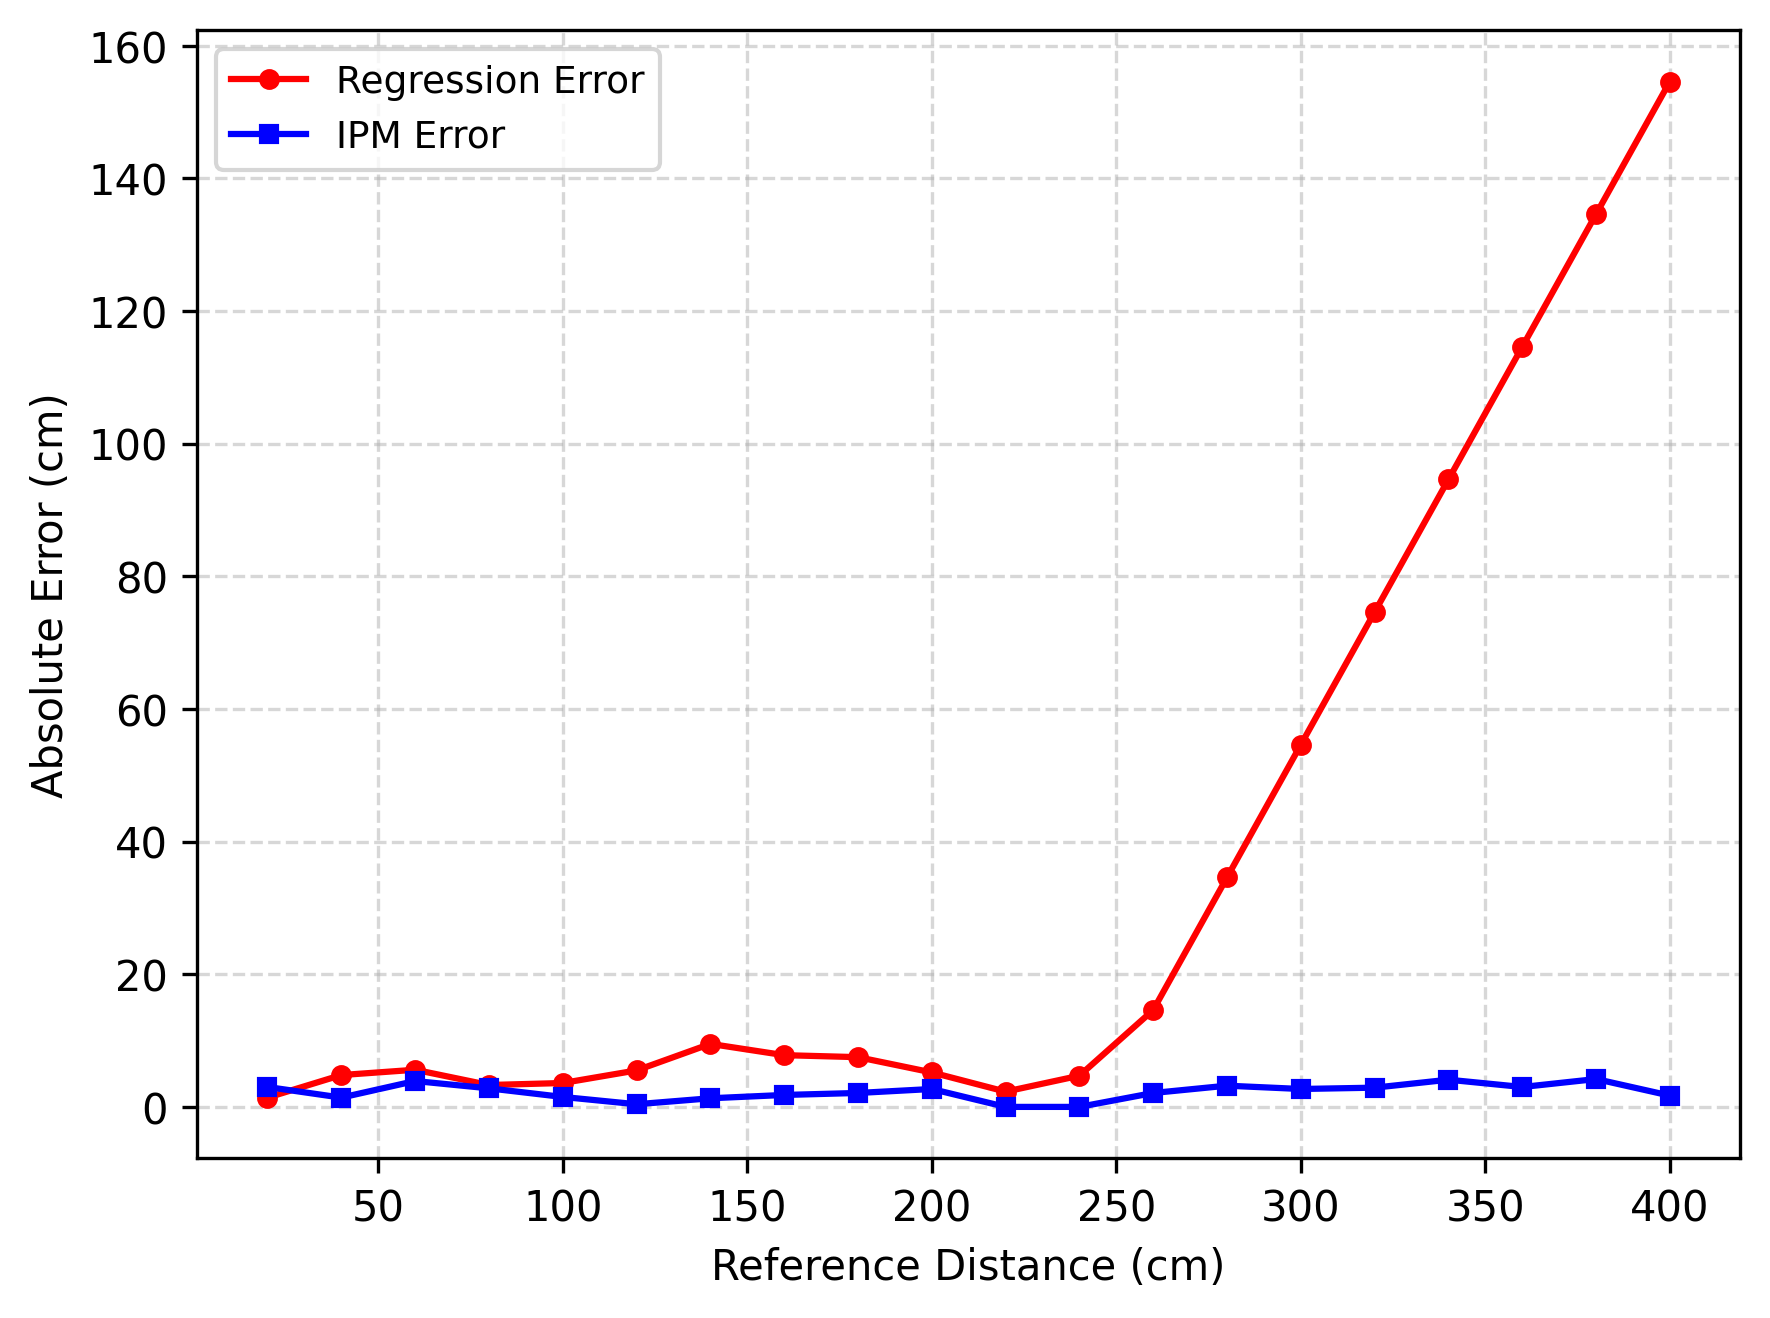
\includegraphics[width=\textwidth]{regression_vs_ipm_error.png}
\\ \vspace{1mm} \footnotesize (b) Absolute distance error.
\end{minipage}
\caption{Comparison between the regression-based and IPM-based distance estimation
methods: (a) estimated distances versus ground-truth distances, and (b) corresponding
absolute distance errors.}
\label{fig:regression_vs_ipm}
\end{figure*}

\subsection{Comparison with Regression-Based Method}

To evaluate the proposed IPM approach, a comparison was conducted with the regression-based
distance estimation method previously used by the ICHIRO ITS team. The evaluation was performed 
in a static setup with the ball placed at distances ranging from 20~cm to 400~cm. Both methods 
estimated the ball distance while the robot actively tracked the target to ensure consistent observations.

The experimental setup is illustrated in Figure~\ref{fig:regression_vs_ipm_setup}, 
and the resulting distance estimates and absolute errors across the tested range are 
presented in Figure~\ref{fig:regression_vs_ipm}.

\begin{figure}[h]
\centering
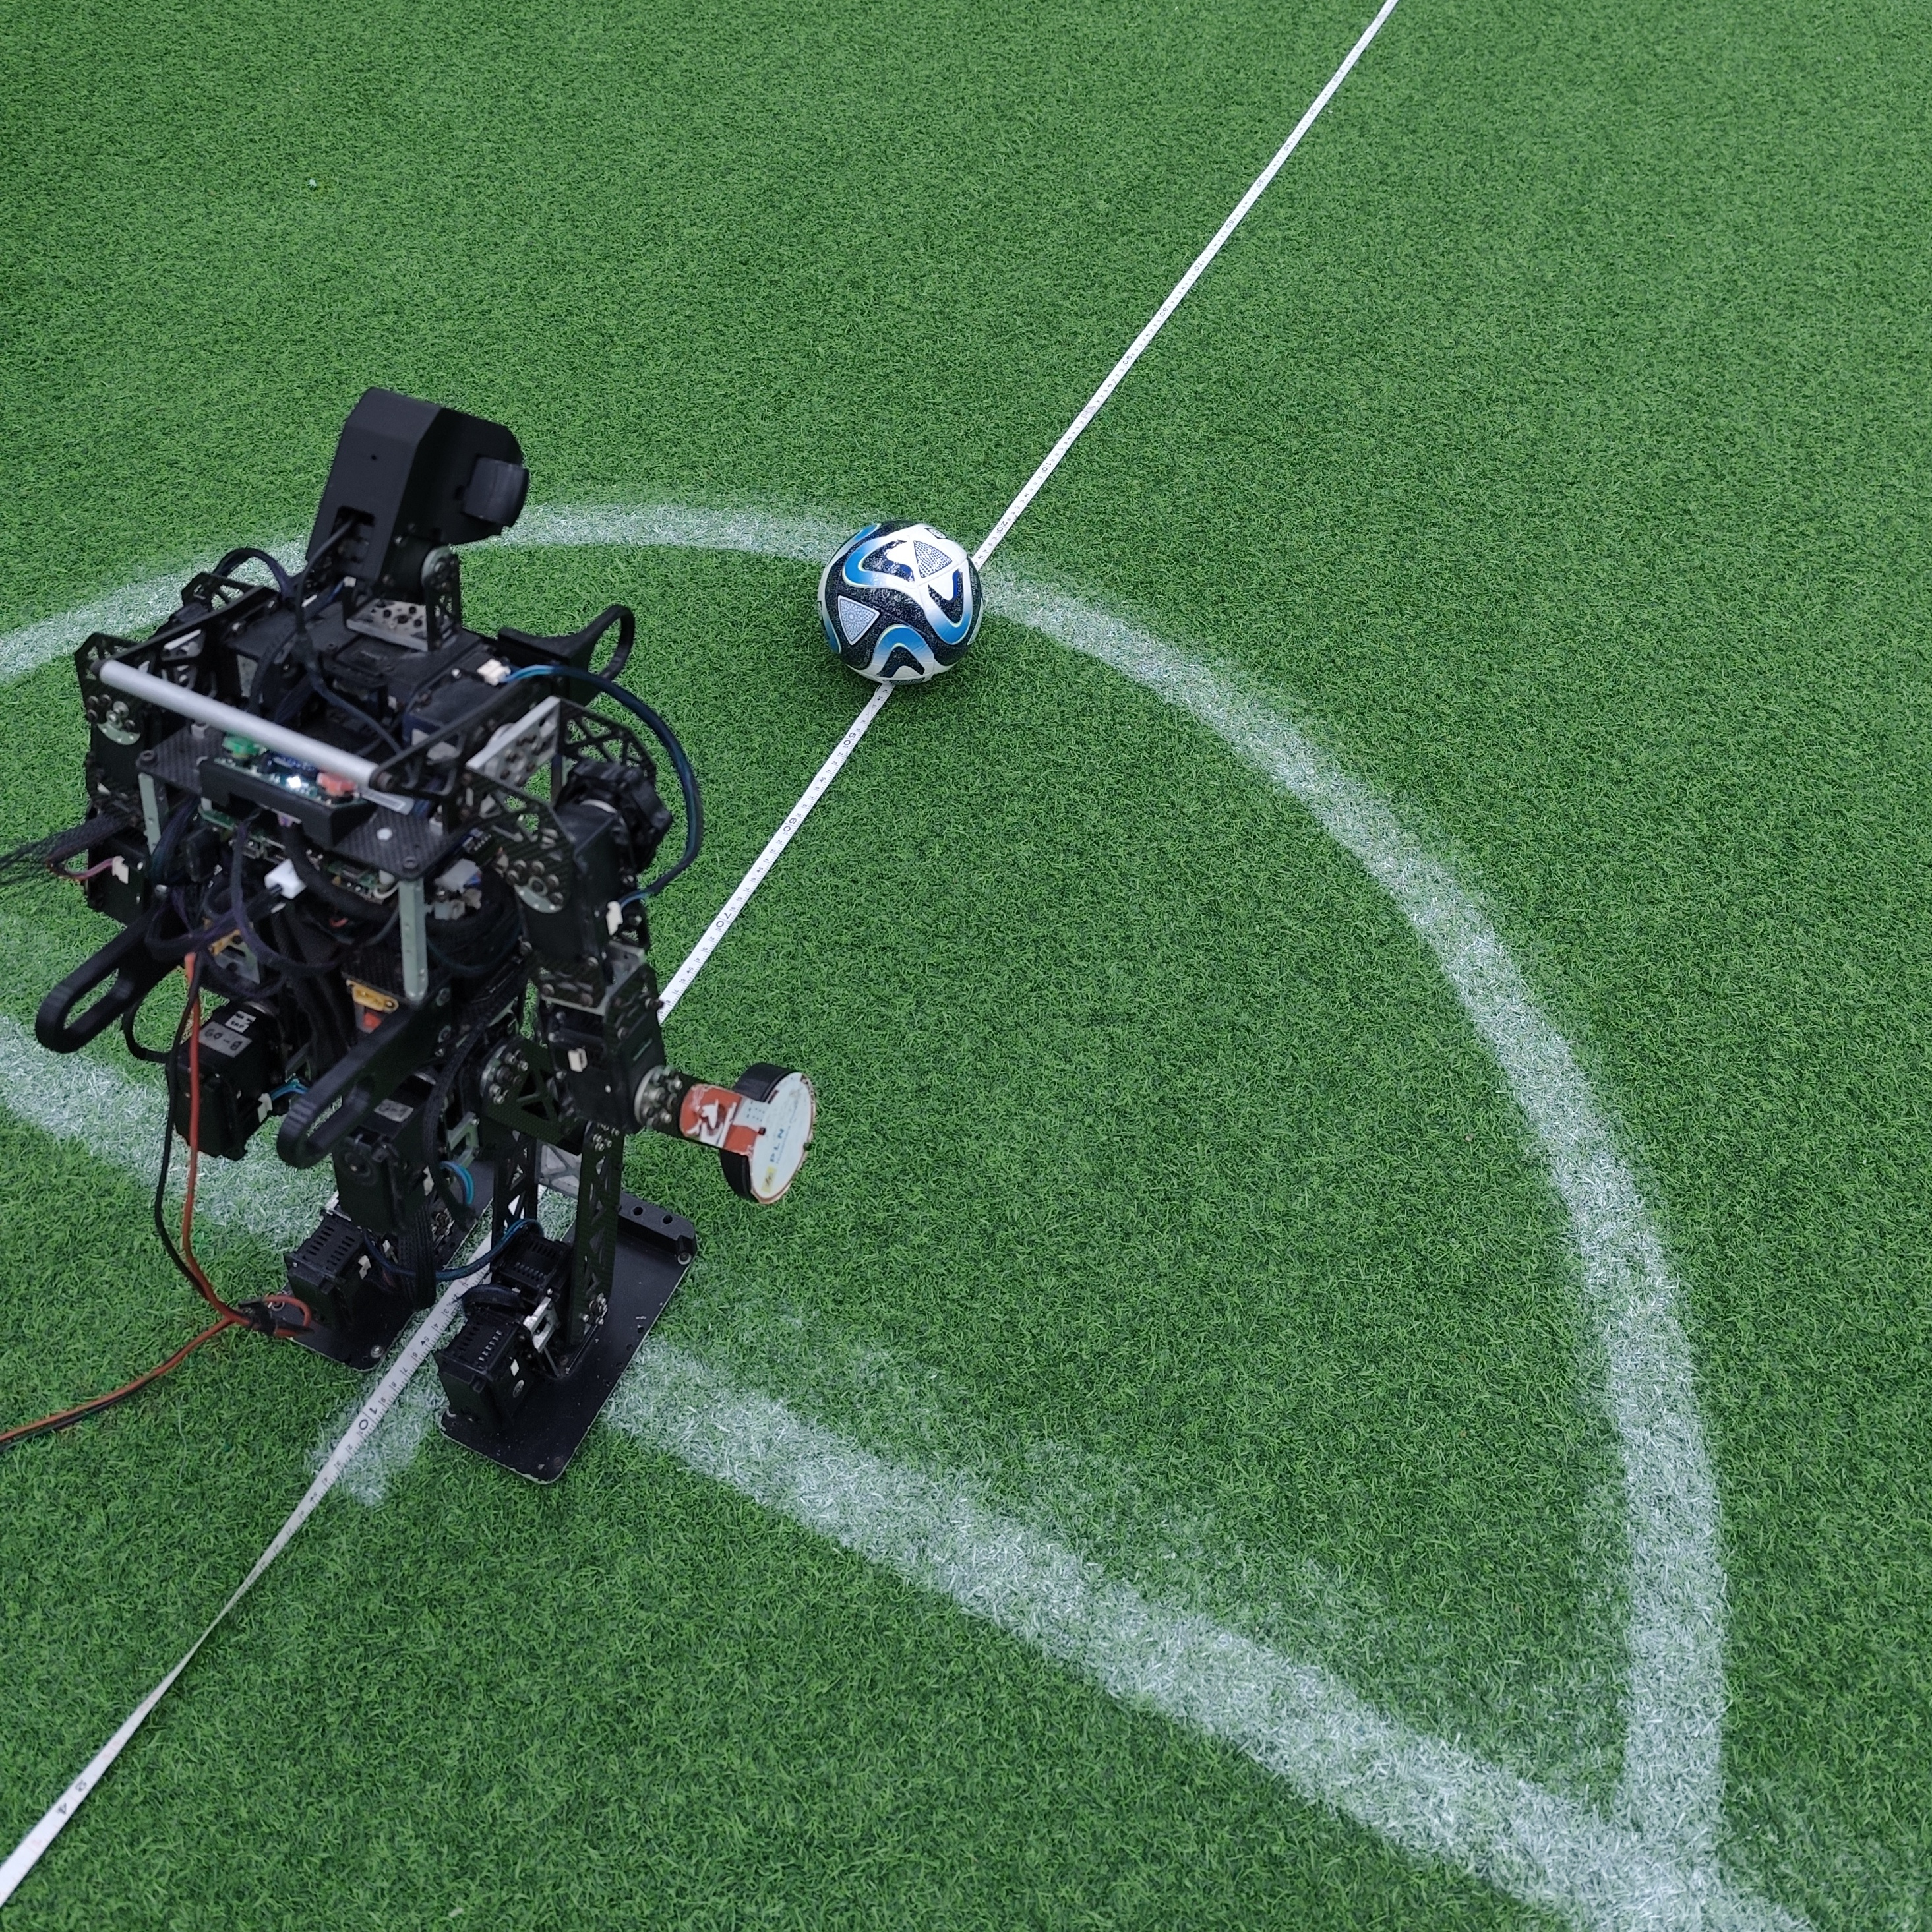
\includegraphics[width=0.8\columnwidth]{regression_vs_ipm_setup.jpg}
\caption{Actual experimental setup for comparing regression-based and IPM distance estimation.}
\label{fig:regression_vs_ipm_setup}
\end{figure}

As shown in Figure~\ref{fig:regression_vs_ipm}a, the regression-based method produces 
acceptable performance at short distances but completely fails to generalize beyond 
approximately 250~cm. At longer ranges, the estimated distance saturates and no longer 
follows the reference trend. This limitation arises because the regression model relies 
primarily on the head tilt angle as its input feature; once the target moves far enough 
that the tilt angle reaches $0^\circ$, the model loses its predictive capability entirely.

In contrast, the proposed IPM method maintains a tight linear relationship with the reference 
distance across the entire 400~cm range. Even at these longer distances, where the regression 
method fails, the IPM estimates continue to track the ground truth accurately, with a maximum 
absolute error of only 4.20~cm. This demonstrates that the proposed IPM approach significantly 
extends the effective perception range of the robot while maintaining high accuracy, providing 
greater reliability for dynamic soccer environments.

\newpage

\section{Conclusion}

In this paper, we implemented Inverse Perspective Mapping (IPM)-based
object position estimation system on a humanoid soccer robot developed
by ICHIRO ITS team using ROS 2. The proposed approach integrates camera calibration,
real-time kinematic transformations, and object detection outputs to estimate
object positions from monocular vision.

Experimental results demonstrate accurate and stable performance under
static conditions. For nearby and intermediate-distance (below 4~m) targets,
the system achieved MAE values below 8~cm, while the lowest error was obtained
for the ball ($O_1$) with an MAE of 1.61~cm. Estimation accuracy decreased for
distant objects due to the increased sensitivity of IPM near the image horizon,
with the largest error observed for the goalpost ($O_6$), which achieved an MAE of
38.80~cm.

During walking, the error distribution became highly non-normal due to
occasional large estimation failures. Nevertheless, the median errors
remained relatively low at 12.74~cm, 14.75~cm, and 5.11~cm for the
ball, robot, and X-intersection, respectively. Furthermore, 59.5\%,
50.2\%, and 62.2\% of the corresponding estimates remained within
15 cm of the reference position, indicating that most object position
estimates remained reasonably accurate despite robot motion.

A comparison with the regression-based method previously used by the ICHIRO ITS 
team demonstrated that the proposed analytical IPM approach eliminates distance 
estimation saturation, successfully extending the reliable perception range from 
250~cm to 400~cm with a maximum absolute error of only 4.20~cm. Furthermore, 
unlike the regression-based approach, the proposed method does not depend on active 
object tracking or repeated empirical distance calibration, making it highly robust 
and suitable for deployment in dynamic humanoid soccer environments.

Future work will focus on integrating the proposed system with higher-level perception
modules, such as localization and mapping, as well as improving robustness against
detection noise, joint offsets, and IMU drift.

% >>>>>>>>>>>>>>>>>>>>>> Bibliography <<<<<<<<<<<<<<<<<<<<<<<<<<<<<<<<<<<<<

\bibliographystyle{BibTeXtran}   % (uses file "BibTeXtran.bst")
\bibliography{BibTeXrefs}       % (expects the reference in the file "BibTeXrefs.bib")

\end{document}
